\chapter{Jaynes-Cummings de dos átomos, no lineal, medio Kerr}
\label{ch4_dinamica}

%CAMBIAR ESTO PARA PERSONALIZARLO A MI GUSTO
\pagestyle{fancy}
\fancyhf{}
\fancyhead[LE]{\nouppercase{\rightmark\hfill}}
\fancyhead[RO]{\nouppercase{\leftmark\hfill}}
\fancyfoot[LE,RO]{\hfill\thepage\hfill}

En este capitulo se extiende el modelo de Jaynes-Cummings presentado en el capitulo \ref{ch3_jcm}, agregandole nuevas cosas. Lo mas importante es que ahora vamos a tener dos átomos dentro de una misma cavidad. En la literatura en general, el JCM fue extendido para considerar dos cavidades donde cada una tiene su propio átomo, y usando una condición inicial entrelazada se puede hacer interactuar ambas cavidades REFS. El camino que se tomó en este trabajo, es un tanto fuera de lo convensional ya que no hay muchos estudios sobre este sistema. El principal obstaculo que presenta este problema, es que el espacio de Hilbert crece mucho y se torna inmanejable analiticamente; como bien ya sabemos, el JCM tiene subespacios de 2 dimensiones que no se mezclan, y utilizando esta estrategia vamos a ver que en este caso tenemos subespacios de 4x4 que tampoco se mezclan en el caso unitario. Esto nos permite encontrar algunas expresiones analiticas, pero en general se utilizaran métodos númericos para analizar la dinamica. \newline
Este capitulo entonces seguira un hilo conductor, partiendo desde el caso mas sencillo hasta llegar a analizar cuales son los efectos de los diferentes parámetros en el problema. 
	Primero vamos a considerar una cavidad perfecta, es decir sin disipaci\'on, agregandole el segundo átomo, vamos a intentar de entender cual es el efecto de este sobre el modelo de un solo átomo. Para esto haremos un analisis poblacional, y de observables como la entropia reducida, la concurrencia, las matrices de pauli. Una vez agregado el segundo átomo, vamos a prender las interacciones de a una y vamos a analizar cuales son sus efectos. Luego, vamos a comparar esto con el caso en donde la cavidad presenta perdidas. Principalmente, nos centraremos en un analisis del entrelazamiento, ya que esta es la cualidad mas interesante que tenemos en el ambito de la informaci\'on cu\'antica. 

\textcolor{blue}{Luego, se analizar\'a el problema para dos átomos, primero en el caso que estos no interact\'uan
directamente entre si, sino que lo hace indirectamente a travez de la cavidad. La comparativa entre
esta situación y la mas comun, donde los átomos interactuan mediante sus espines o sus momentos
dipolares, es muy rica porque nos permite discernir con claridad cual es el efecto de la cavidad
y cual de la interacción entre los átomos a la hora de entrelazarse e intercambiar energía.
El problema de dos átomos tiene una peculiaridad al elegir las condiciones iniciales, ya que la
dinamica depende de esta eleccion, y hay muchas diferentes configuraciones interesantes, por un lado
por la gran dimension del espacio, y por otro lado, esta la posibilidad de jugar con las simetrias.
Surge asi la pregunta de si es importante, o si tiene sentido, teniendo dos átomos indistinguibles
en una cavidad, que la condición inicial sea asimetrica ante intercambio. 
}

\section{Modelo de dos átomos y solucion unitaria}
En este trabajo, nos vamos a concentrar en una extension del modelo, donde vamos a ubicar dos átomos dentro de la cavidad. Estos átomos pueden interactuar entre si, y con la cavidad, y ademas agregaremos no-linealidades en el acoplamiento y en el medio.
Vamos a usar un modelo de Jaynes-Cummings para describir la interacci\'on entre el campo electromagn\'etico y los átomos. Adem\'as supondremos que el acoplamiento depende de la cantidad de fotones y los átomos podr\'an interactuar entre si mediante un termino tipo Ising y otro tipo dipolo-dipolo. Recordemos que para estamos asumiendo que vale la aproximaci\'on de onda rotante ($\omega_0 \sim \omega$) y $g << \omega,\omega_0$.
Entonces, el Hamiltoniano que describe este problema es el siguiente:

\begin{equation}
\begin{split}
     \hat H & =\underbrace{\hbar \omega_0 h(\hat n) \hat n }_{\hat H_F}+\underbrace{\frac{\hbar \omega}{2}(\hat\sigma_Z^{(1)}+\hat\sigma_Z^{(2)})}_{\hat H_A}   \\ 
     & + \underbrace{\hbar g(\hat\sigma_+^{(1)}\hat a f(\hat n)+\hat\sigma_-^{(1)}f(\hat n) \hat a^\dagger + \hat\sigma_+^{(2)}\hat a f(\hat n)+\hat\sigma_-^{(2)}f(\hat n) \hat a^\dagger)}_{H_{FA}} + \\ & \underbrace{2\hbar \kappa (\hat \sigma_-^{(1)}\hat \sigma_+^{(2)}+\hat \sigma_+^{(1)}\hat \sigma_-^{(2)}) + \hbar J \hat \sigma_Z^{(1)}\hat \sigma_Z^{(2)}}_{H_{AA}}
\end{split}
\end{equation}

donde $\hat a$ es el operador de aniquilaci\'on del fot\'on, $\omega_0$ y $\omega$ son las frecuencias del fot\'on y del átomo respectivamente, $g$ es la constante de acoplamiento, las constantes $J$ y $\kappa$ son los par\'ametros de Ising y de dipolo-dipolo para las interacciones átomo-átomo, y los operadores $\sigma^{(i)}$ son las matrices de Pauli que act\'uan sobre el átomo i-esimo. Finalmente, las funciones $h(\hat n)$ y $f(\hat n)$ son las que van a dar cuenta de la no linealidad dependiente del numero de fotones de la cavidad $\hat n = \hat a^\dagger \hat a$. 

Tomando un medio tipo Kerr la funci\'on $h(\hat n)=1+\frac{\chi}{\omega_0}\hat n$ \cite{}\textcolor{red}{(CITA)}, y la funci\'on $f(\hat n) =1$ si tomamos un acoplamiento lineal, y $f(\hat n) = \sqrt{\hat n}$ si consideramos un acoplamiento tipo Buck-Sukumar \cite{}\textcolor{red}{(CITA)}

En este punto es normal hacer una transformaci\'on unitaria  $K = \exp\left\{-i \omega t (\hat a^\dagger a + \sigma_z/2)\right\}$ para dejar el Hamiltoniano en funci\'on del Detuning $\Delta (\sim 0)$. 

\begin{equation}
\begin{split}
     \hat H_I & =\hbar \chi \hat n^2+\frac{\hbar \Delta}{2}(\hat\sigma_Z^{(1)}+\hat\sigma_Z^{(2)})   \\ 
     & + \hbar g(\hat\sigma_+^{(1)}\hat a f(\hat n)+\hat\sigma_-^{(1)}f(\hat n) \hat a^\dagger + \hat\sigma_+^{(2)}\hat a f(\hat n)+\hat\sigma_-^{(2)}f(\hat n) \hat a^\dagger) \\ 
 & + 2\hbar \kappa (\hat \sigma_-^{(1)}\hat \sigma_+^{(2)}+\hat \sigma_+^{(1)}\hat \sigma_-^{(2)}) + \hbar J \hat \sigma_Z^{(1)}\hat \sigma_Z^{(2)}
\end{split}
\end{equation}\label{eq4:H}
Este es el Hamiltoniano con el que vamos a trabajar, asi que a partir de ahora vamos a olvidarnos del subindice I. Obsérvese que el caso de $\chi=0$ es el caso de un medio lineal. 
\textcolor{blue}{ACA PUEDO AGREGAR UN ESQUEMA DE COMO SERIA.} En este esquema se ve como seria el experimento planteado. 

Este Hamiltoniano se puede resolver analiticamente para el caso de una cavidad sin perdidas. En analogia con el caso de 1 átomo, vamos a elegir la base de N excitaciones, donde esperamos que estos subespacios queden invariantes, es decir, que el Hamiltoniano sea diagonal por bloques, pero como ahora tenemos 2 átomos, tenemos que elegir una base que respete simetrias, para N excitaciones los estados de la base son $\left\{\ket{ggn},\frac{1}{\sqrt{2}}(\ket{eg,n-1}+\ket{ge,n-1}),\ket{ee,n-2},,\frac{1}{\sqrt{2}}(\ket{eg,n-1}-\ket{ge,n-1})\right\}$. En esta base, el Hamiltoniano se diagonaliza por bloques y el bloque de N excitaciones queda
El problema unitario se puede resolver analíticamente. Esto esta hecho en el paper de los autores \textit{O de los Santos-Sánchez
, C González-Gutiérrez and J Récamier}, titulado \textit{Nonlinear Jaynes–Cummings model for two
interacting two-level atoms} \cite{paper:santos}\textcolor{red}{(CITA)}. 
\textcolor{red}{Ac\'a tengo que pasar las cuentas a latex, pero las hice en papel para ver si entend\'ia todo.}
Para resolver el problema lo primero que hacemos es notar que el Hamiltoniano conserva el numero de exitaciones, es decir $[H,\hat N]=0$, y en esta situación es sabido que el Hamiltoniano de JC es diagonal por bloques si elegimos convenientemente la base, esta es la que agrupa los estados con misma cantidad de excitaciones $\hat N = \hat n + \hat \sigma_+^{(1)}\hat \sigma_-^{(1)}+\hat \sigma_+^{(2)}\hat \sigma_-^{(2)}$: 
\begin{equation}
\begin{split}
    & \left\{\ket{\Phi^{(n)}_1}=\ket{ggn},\ket{\Phi^{(n)}_2}=\frac{1}{\sqrt{2}}(\ket{egn-1}+\ket{gen-1}),\ket{\Phi^{(n)}_3}=\ket{een-2},\right. \\
& \left. \ket{\Phi^{(n)}_4}=\frac{1}{\sqrt{2}}(\ket{egn-1}-\ket{gen-1})\right\} 
\end{split}
\label{ec4:base}
\end{equation}
,donde se eligi\'o esta combinaci\'on particular porque el ultimo estado de la base, que es impar ante intercambio, queda desacoplado de los otros, simplificando el problema. Esto se ve al evaluar los elementos de matriz del Hamiltoniano $H_{i,j}=\bra{\Phi_i}\hat H \ket{\Phi_j}$, este queda en bloques, y el subespacio correspondiente a $n$ excitaciones $\hat H^{(n)}$ es una matriz de 4x4
\begin{equation}
    \frac{\hat H^{(n)}}{\hbar}=
    \begin{pmatrix}
     \chi n^2 - \Delta +  J & \sqrt{2} g f(n)\sqrt{n} & 0 & 0 \\
    \sqrt{2} g f(n)\sqrt{n} &  \chi (n-1)^2  -  J + 2 k & \sqrt{2} g f(n-1)\sqrt{n-1} & 0 \\
    0 & \sqrt{2} g f(n-1)\sqrt{n-1} &  \chi (n-2)^2 +  \Delta +  J & 0 \\
    0&0&0& \begin{aligned} 
                 & \chi (n-1)^2  \\ 
                 &-  J - 2 k
        \end{aligned}
    \end{pmatrix}
\end{equation}
Vemos claramente que el estados impar ante intercambio esta aislado, y entonces es autoestado del problema, y por lo tanto evoluciona solo y no se mezcla con los otros estados. Esto nos sirve porque ahora, para terminar de resolver el problema, tenemos que diagonalizar la matriz de 3x3. Cabe aclarar que esta matriz solo es valida para $n\geq 2$, ya que los subespacios con $N=0,1$ no tienen 4 estados. En estos casos la soluci\'on del problema de autovalores es mas sencilla aun, as\'i que solo dejaremos los resultados. A partir de ahora se usar\'a como convención $\hbar=1$. \newline
Para resolver el problema de autovalores de la matriz de 3x3 utilizamos la fórmula de Cardano para conseguir las ra\'ices triples que nos aparecen en el polinomio caracter\'istico, y entonces encontramos que los autovalores son
\begin{equation}
    E_j^{(n)}=-\frac{1}{3}\beta_n+2\sqrt{-Q_n}\cos{\left(\frac{\theta_n+2(j-1)\pi}{3}\right)}
    \label{ec4:autoenergias}
\end{equation}
para $j=1,2,3$, y donde 
\begin{equation}
    \theta_n=\cos^{-1}\left(\frac{R_n}{\sqrt{-Q_n^3}}\right)
\end{equation}
\begin{equation}
    \begin{aligned}
        Q_n & = \frac{3\gamma_n-\beta_n^2}{9} \\
        R_n & = \frac{9\beta_n\gamma_n-27\eta_n-2\beta_n^3}{54} \\
        \beta_n & = - \left( \chi(n^2+(n-1)^2+(n-2)^2)+J+2k\right) \\
        \gamma_n & = (\chi(n-1)^2 - J + 2k)(x(n-2)^2+\chi n^2+2J) \\ 
        & +(\chi (n-2)^2+\Delta+J)(x n^2-\Delta+J)-2g^2(n^{2a}+(n-1)^{2a}) \\ 
        \eta_n &= -(\chi n^2-\Delta+J)(\chi(n-2)^2+\Delta+J)(\chi(n-1)^2-J+2k) \\
        &+2g^2 \left[  \chi(n-2)^2n^{2a}+\chi n^2(n-1)^{2a}+\Delta\left(n^{2a}-(n-1)^{2a}\right) +J(n^{2a}-(n-1)^{2a})\right]
    \end{aligned} 
    \label{ec4:parametros solucion}
\end{equation}
donde $a=\frac{1}{2}$ se corresponde con acoplamiento lineal, es decir, $f(n)=1$, y $a=1$ a Buck-Sukumar $f(n)=\sqrt{n}$. Los autovalores ser\'an reales si $Q_n^3+R_n^2<0$.
Con esto podemos escribir los autovectores:
\begin{equation}
    \begin{split}
        \ket{u_j^{(n)}} &= \frac{1}{N_j^{(n)}} \bigg[ \left((E_j^{(n)} - H_{22}^{(n)})(E_j^{(n)}-H_{33}^{(n)}) - H_{23}^{(n)^2} \right) \ket{\Phi_1^{(n)}} \\ &+ H_{21}^{(n)}(E_j^{(n)}-H_{33}^{(n)})\ket{\Phi_2^{(n)}} + H_{23}^{(n)}H_{12}^{(n)}\ket{\Phi_3^{(n)}}\bigg]
    \end{split}
\end{equation}
Obviamente no nos olvidemos del estado $\ket{\Phi_4^{(n)}}$, que tambi\'en es autoestado, con autovalor $E_4^{(n)}=\chi(n-1)^2-J-2k$.
Para el subespacio de $N=0$ solo tenemos un vector $\ket{\Phi_1^{(0)}}=\ket{gg0}$ y su autovalor es $E_1^{(0)}=-\Delta+J$.
Para $N=1$ tenemos 3 vectores en el subespacio, y las autoenergias son
\begin{align}
    E_{1,2}^{(1)} &=\frac{\chi -\Delta}{2} +k \pm \sqrt{2g^2+(k-J+\frac{\Delta -\chi}{2} )^2} \\
    E_3^{(1)} & = -2k-J 
\end{align}
y sus autovectores
\begin{align}
    \ket{u_{1,2}^{(1)}}&=\frac{1}{N_{1,2}^{(1)}}(-\sqrt{2}g\ket{gg1}+ \left(\frac{\chi-\Delta}{2}+J-k \mp \sqrt{2g^2+(k-J+\frac{\Delta -\chi}{2} )^2} \right)\dfrac{\ket{eg0}+\ket{ge0}}{\sqrt{2}}\\
    \ket{u_3^{(1)}}&= \frac{1}{\sqrt{2}}(\ket{eg0}-\ket{ge0})
\end{align}
Con esto, podemos resolver analíticamente la evolución temporal de cualquier estado inicial.
Para esto solo tenemos que desarrollar el estado inicial en terminos de los autovectores, y la evolución temporal esta dada por
\begin{equation}
\ket{\psi(t)}=e^{-iHt}\ket{\psi(0)}=\sum_{j,n} c_j^{(n)}e^{-iE_j^{(n)}t}\ket{u_j^{(n)}}
\end{equation}
donde $c_j^{(n)}=\braket{u_j^{(n)}}{\psi(0)}$.
La complejidad de estas expresiones hace complicado conseguir conclusiones interesantes,aun asi, algo que se puede notar, es la diferencia fundamental que se encuentra para las energias con un numero total de excitaciones $N=1$ y $N>1$. Si se observa el factor que esta antes de la raiz cuadrada,  se ve que para el caso en que $N \geq 2$ tenemos un $\frac{1}{3}\beta_n$ que solo depende de $\chi$, $J$, $k$ y $n$. Mientras tanto, en el caso de $N=1$, este factor depende del detunning $\Delta$. Esto es interesante, ya que uno podria pensar que la formula para $N$ excitaciones se puede generalizar para incluir $N=0,1$, pero la fundamental diferencia de tener mas o menos estados que interactuan entre si, da lugar a efectos fundamentalmente diferentes. Si uno mira en detalle las cuentas, se percata de que en el caso de $N=1$ este factor $\Delta$ aparece, ya que en la matriz Hamiltoniana el unico estado con $N=1$ que tiene un termino que incluye al detunning, es el estado $\ket{gg1}$, y los otros dos estados al ser un átomo excitado y otro no, el termino de detunning se cancela. Por lo tanto, este termino con $\Delta$ sobrevive, al contrario que en todos los demas subespacios, ya que tenemos por un lado el termino del $\ket{ggn}$ que nos aporta un $\Delta$, y el termino de $\ket{ee,n-2}$ que nos aporta otro $\Delta$ pero con el signo cambiado, y elimina la contribución del primer estado a la energía. Esto es super interesante, ya que para $N=1$, si aumentamos el detunning, no solo se separan los niveles de energía, sino que tambien hay una asimetria por el termino independiente. Para analizar esto en detalle, en la figura \ref{fig:relación energia detunning} se observan las energias de los diferentes niveles en función del detunning. 

\begin{figure}
    \centering
    \begin{subfigure}[h]{0.49\textwidth}
        \centering
        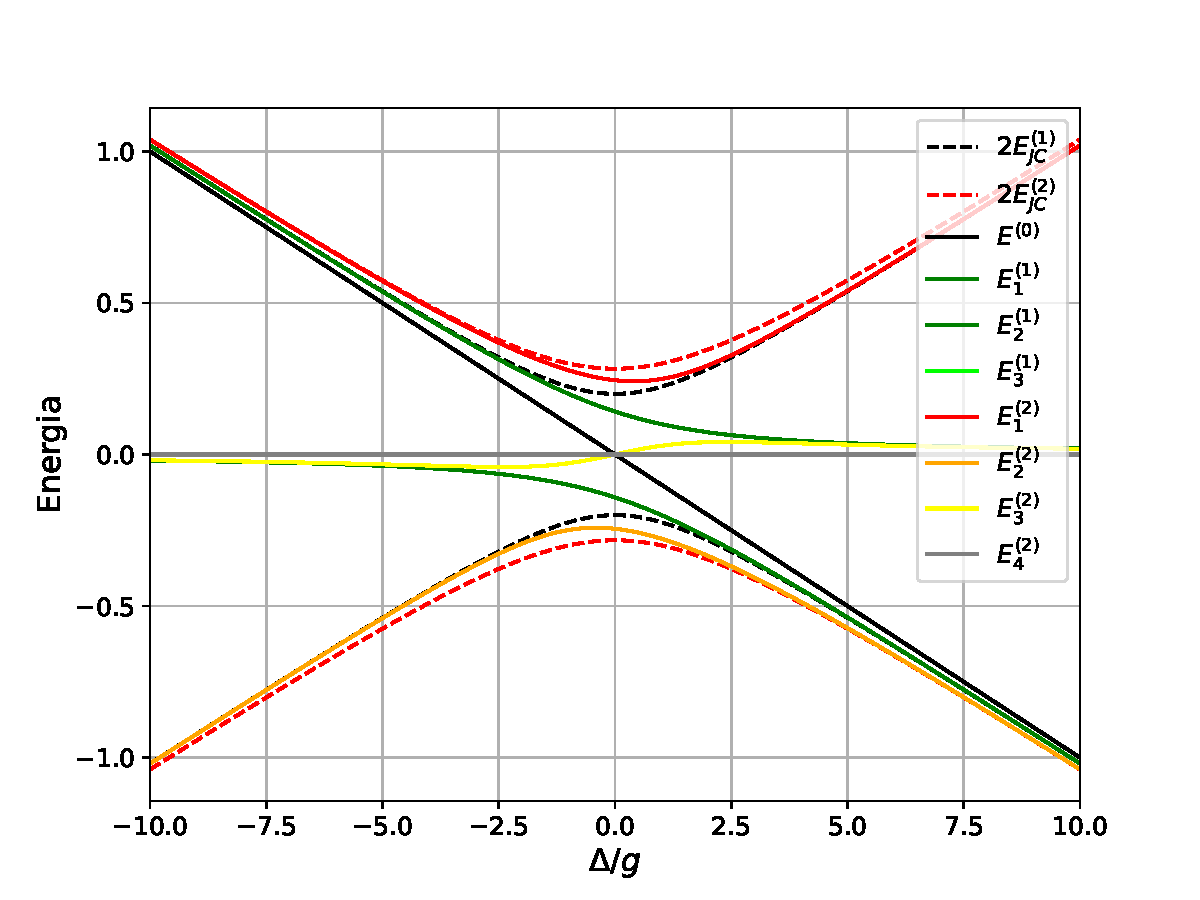
\includegraphics[width=\textwidth]{figuras/ch4/relacion_energia_detunning1.pdf}
        \caption{$k=J=0$}
        \label{fig:relación energia detunning 1}
    \end{subfigure}
    \hfill
    \begin{subfigure}[h]{0.49\textwidth}
        \centering
        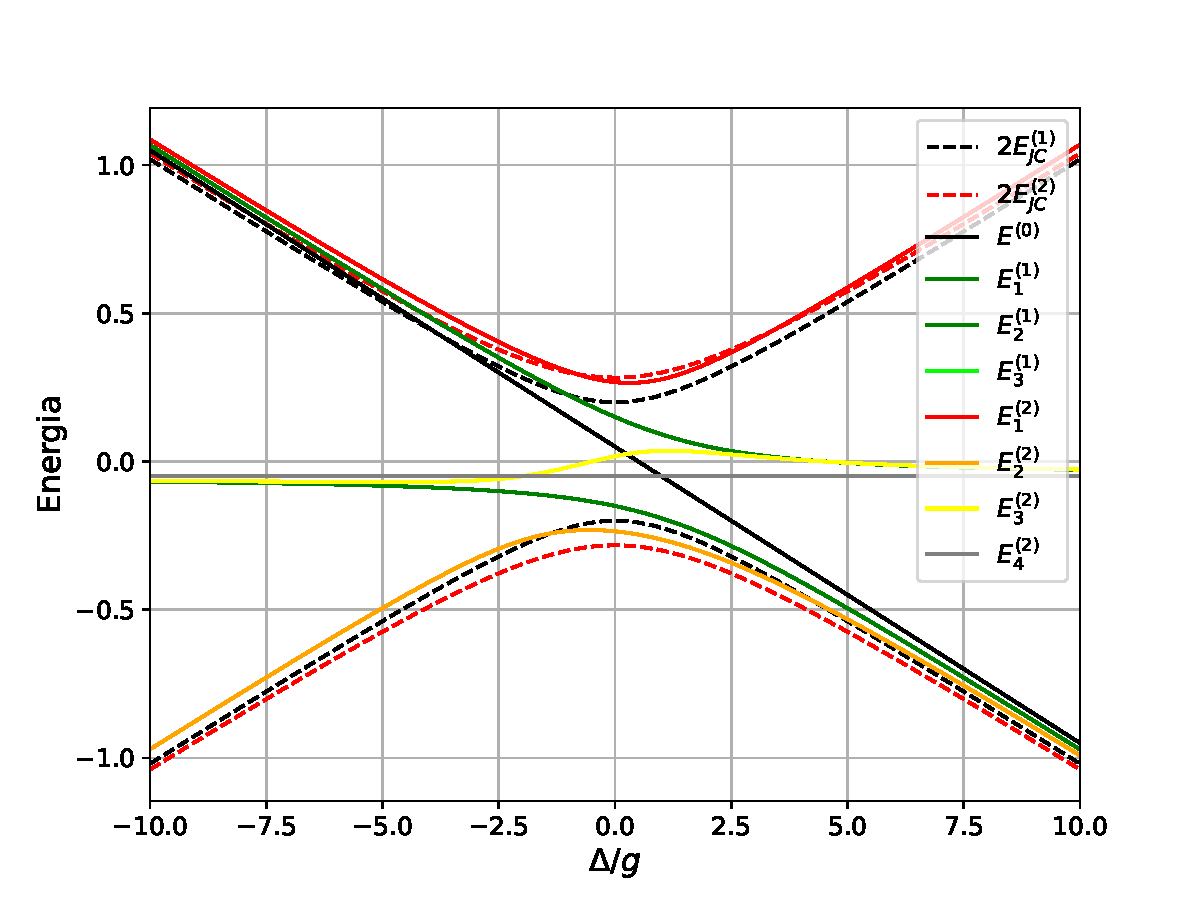
\includegraphics[width=\textwidth]{figuras/ch4/relacion_energia_detunning2.pdf}
        \caption{$J\neq 0$}
        \label{fig:relación energia detunning 2}
    \end{subfigure}
       \caption{Relación entre energía y detunning para los diferentes niveles de energía del problema. Las lineas solidas muestran la energía de los estados del JC doble con N=0 (negro, solido), N=1 (verde oscuro y lima, solido) y N=2 (rojo, naranja, amarillo y gris; solido). Tambien se muestran los niveles de energía del JC de un átomo para N=1 (negro; rayado) y N=2 (rojo; rayado). Observese que las energias del JC de un átomo estan multiplicadas por 2.}
       \label{fig:relación energia detunning}
\end{figure}
En esta figura \ref{fig:relación energia detunning 1} se observan las energias de los primeros niveles para el modelo de un átomo, mostrados con lineas rayadas, y de dos átomos, con lineas solidas; para esta figura se tomaron átomos que no interactuan ($k=J=0$) y una cavidad lineal ($\chi=0$). Se puede ver que, si bien el modelo de dos átomos tiene estructuras mas complicadas, son similares a las de 1 átomo. En primer lugar, los estados con N=2 (rojo y naranja; solido) tienen una forma igual a la de JC de 1 átomo, si bien esta un poco desfasada, es interesante ver como las lineas tienen una coincidencia muy grande, recordando que en el grafico las lineas rayadas estan multiplicadas por 2, esto nos da una interpretación bastante buena, y es que la energía de dos átomos no interactuantes en una cavidad es igual (o muy parecida) a dos veces la energía de 1 átomo en una cavidad. \textcolor{red}{Esto tengo que chequear con cuentas} \textcolor{blue}{Creo que esto se debe al corrimiento Lamb, ya que ahora tenemos dos átomos que interactuan con el vacio, entonces el corrimiento es 1 unidad mas grande en los extremos, que es justamente lo que vemos en el grafico, cuando el detunning es muy negativo, la energ\'ia tiende a ser igual a la de un JC simple con 2 excitaciones, y cuando el detunning es muy positivo, entonces tiende a la de 1 excitaci\'on; esta asimetr\'ia para $\Delta>0$ y $\Delta<0$ se observar\'a en resultados posteriores.} Por otro lado, se puede observar lo que se habia comentado anteriormente, que la energ\'ia de los estados con $N=1$ tienen un t\'ermino fuera de la raiz, que hace que sea mas asim\'etrico a\'un. Normalmente, en el JC de 1 átomo, ya que todos los niveles de energía tienen una forma funcional igual, este termino de afuera de la raiz se le puede agregar o quitar como un offset en la energía del estado fundamental, la diferencia con este caso es que, no todos los niveles de energía presentan esto, entonces si agregamos un offset, igualmente habria una diferencia. 

Otra cosa interesante de notar es que si la cavidad es lineal, entonces los estados antisimetricos de diferentes excitaciones $\frac{1}{\sqrt{2}}(\ket{eg,n}-\ket{ge,n})$ y $\frac{1}{\sqrt{2}}(\ket{eg,n'}-\ket{ge,n'})$, estan degenerados en energía.

Una vez estudiados los niveles de energía y comparados con el caso de 1 átomo, vamos a proseguir con la dinámica del problema, que en el caso unitario puede resolverse analíticamente, pero a\'un asi, nos concentraremos en simulaciones numéricas.
Para comenzar, vamos a intentar de recuperar el caso de un átomo, asimetrizando el acoplamiento uno de los dos átomos que tenemos en la cavidad, y haciendo tender este a cero, es decir, vamos a trabajar con $k=J=0$ y vamos a agregar un parámetro adimensional $\alpha$ que solamente actúa sobre el átomo 2, y sirve de apantallamiento. Este parámetro $\alpha$ acompañara a las constantes de acoplamiento, por ejemplo el acoplamiento entre el átomo y la cavidad $g\rightarrow g\alpha$, tal que si $\alpha \rightarrow 0$ entonces el átomo quedara desacoplado de la cavidad. 

\section{Dinámica con apantallamiento}

Lo primero que se tiene que hacer es recuperar los resultados anteriores. Para aclarar, en la figura \ref{fig4:diagrama esquematico} se muestra un esquema de como es el problema que se esta trabajando, con los nombres que se le darán a las partes del sistema. Llamaremos atomo B al que esta apantallado mediante el parámetro adimensional $\alpha$, el indice A se referirá al otro átomo, y C a la cavidad. Entonces, para recuperar los resultados anteriores, se propone que $\alpha=0$ y la interacción entre los átomos $k=J=0$. De esta manera, se elige en analogía con el caso de 1 átomo, como estado inicial cualquier estado donde el átomo A sea excitado, y la cavidad C no tenga ningún fotón; por lo tanto se elige el estado inicial mas sencillo posible que cumple estas condiciones $\ket{\psi_0}=\ket{eg0}$. Si bien este apantallamiento no tiene un significado fisico, y experimentalmente es imposible lograr estas condiciones, realizar este estudio sirve para entender cualitativamente los efectos de cada parametro del problema, y tambien entender que el entrelazamiento entre los dos atomos, lleva a efectos impredecibles. La complejizacion del problema de 1 atomo al de 2 atomos es muy grande, y por eso es necesario ir de a poco.
\begin{figure}[H]
    \begin{minipage}[c]{0.67\textwidth}
        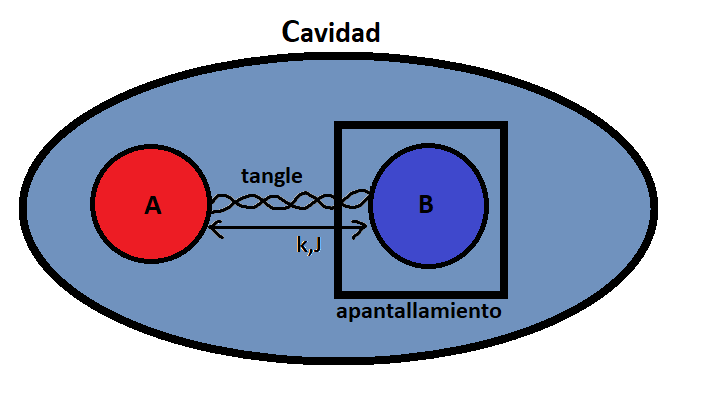
\includegraphics[width=\textwidth]{figuras/ch4/diagrama esquematico.png}
    \end{minipage}\hfill
    \begin{minipage}[c]{0.3\textwidth}
    \caption{Esquema del problema de estudio. Se nombran a las partes para referenciarlas fácilmente. Los átomos los llamamos A y B, donde el átomo B es el que sufre el apantallamiento que utilizaremos para recuperar los resultados anteriores. La cavidad la llamaremos C, esta puede contener una cantidad arbitraria de excitaciones, pero nos concentraremos principalmente en 0,1 y 2 excitaciones. Ambos átomos son de dos niveles, y en principio son idénticos e indistinguibles, pero se le agrega un apantallamiento artificial.
         } \label{fig4:diagrama esquematico}
  \end{minipage}
\end{figure}
Utilizando esta condición inicial se realiza una simulación numérica y se observan las poblaciones, y se espera recuperar la misma dinámica que en el caso de 1 átomo, ya que el átomo B no interactúa con ninguna de las otras partes del sistema A y C. Para poder representar el estado del sistema sobre una esfera de Bloch, se realiza una traza parcial sobre el átomo B, y así se obtiene la figura \ref{fig4:bloch delta}, donde se muestran 3 trayectorias correspondientes a diferentes valores del detunning, la linea azul es el caso resonante $\Delta=0$, y las trayectorias morada y naranja se corresponde con $\Delta=0.5g$ y $\Delta=2g$ respectivamente.
\begin{figure}[H]
    \begin{minipage}[c]{0.67\textwidth}
        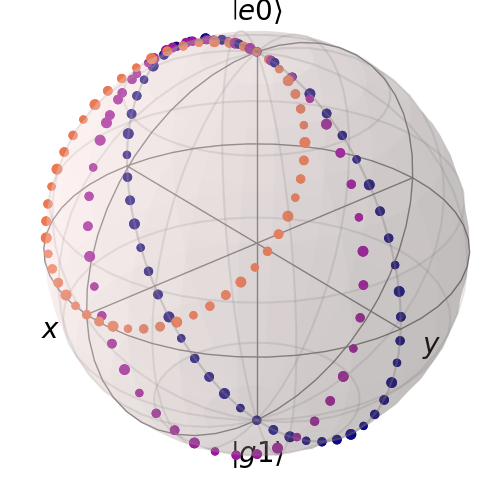
\includegraphics[width=\textwidth]{figuras/ch4/bloch eg0 bloch AC a=0 d=2.0 x=0.0 k=0.0 J=0.0 gamma=0.0 p=0.0.png}
    \end{minipage}\hfill
    \begin{minipage}[c]{0.3\textwidth}
    \caption{
         } \label{fig4:bloch delta}
  \end{minipage}
\end{figure}
Se observa como la dinámica entre estos dos estados es exactamente igual que la observada en la figura \ref{fig3:bloch cinematica}, ademas, como todos los puntos están sobre la superficie de la esfera, los estados son puros, diciéndonos que el estado global es separable, y entonces haber trazado sobre el átomo B no tuvo efecto sobre la dinámica entre el átomo A y la cavidad. Para corroborar esto se realiza un análisis poblacional mas general. \textcolor{red}{hacer gráfico con las probabilidades y ver que la probabilidad de eg0 + gg1 =1}
Lo siguiente que podemos analizar, que no se tenia la posibilidad cuando se tiene 1 átomo, es que se puede considerar una condición inicial entrelazada. Si bien los átomos no interactúan, y el átomo B esta aislado del universo, se puede entrelazar los átomos y luego se apagan las interacciones del átomo B. Por ejemplo, si se considera el estado inicial entrelazado $\ket{\psi_0}=(\ket{eg0}+\ket{ge0})/\sqrt{2}$, se obtiene 
\begin{figure}[H]
    \begin{minipage}[c]{0.67\textwidth}
        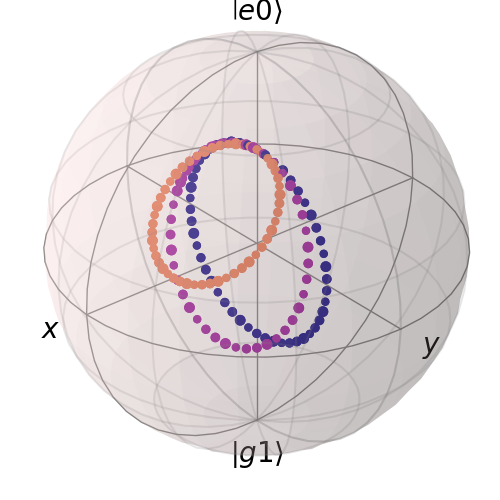
\includegraphics[width=\textwidth]{figuras/ch4/bloch eg0+ge0 bloch AC a=0 d=2.0 x=0.0 k=0.0 J=0.0 gamma=0.0 p=0.0.png}
    \end{minipage}\hfill
    \begin{minipage}[c]{0.3\textwidth}
    \caption{
         } \label{fig4:bloch delta}
  \end{minipage}
\end{figure}
Ahora, los estados no están sobre la superficie, lo que se interpreta como que estamos en presencia de un estado mixto. Al trazar sobre el átomo B, efectivamente se considera como si este fuese parte de un entorno. Al olvidarse de la dinámica del segundo átomo, se puede interpretar como que este se lleva un 50\% de probabilidad de llevarse la excitación, ya que no sabemos si inicialmente el átomo A o el átomo B es el que tiene la excitación. Entonces efectivamente tenemos un 50\% de probabilidad de que el estado de la cavidad sea $\ket{g0}$, y no evoluciona, y un 50\% de probabilidad de que la excitación este dentro de la cavidad, y por lo tanto vemos que la dinámica es la misma que en el caso anterior, pero con amplitudes menores. \textcolor{blue}{ACA IBA A DECIR ALGO, PERO ME PARECE QUE NO PUEDO PORQUE EL ESTADO ENTRELAZADO QUIZAS TIENE ALGUNAS COSAS RARAS. Uno puede adelantarse un poco, y deducir como se comporta la fase geometrica en estos dos casos. Por un lado, en el caso que el estado inicial no este entrelazado, la dinámica es exactamente igual que en el caso de 1 atomo, entonces la fase geométrica es la misma que \ref{eq3:fg unitaria jcm}, en cambio, cuando el estado inicial es el entrelazado, como la dinámica es igual que antes pero con un medio de la probabilidad, y luego el átomo B no evoluciona, entonces es autoestado y no acumula fase geométrica. Por lo tanto se puede concluir que en el caso entrelazado la FG va a ser la mitad que en el caso no entrelazado.}

Para analizar mas en detalle la dinámica, y para poder realizar comparaciones cuando se complejice el problema, se puede realizar un estudio poblacional, y también podemos mirar las entropias relativas y otros observables importantes.
En primer lugar, el caso separable $\psi_0=\ket{eg0}$, es idéntico al caso de 1 átomo, ya que el átomo B no evoluciona por estar totalmente aislado del sistema. Lo único que se puede resaltar es que, si se traza sobre la cavidad, que es algo que es útil para observar el entrelazamiento entre los átomos, lo único destacable es que el estado es mixto, ya que la evolución temporal del sistema átomo A-átomo B consta del atomo B en el estado fundamental $\ket{g}$, y el átomo A oscila entre el estado excitado y fundamental. La amplitud de oscilación y el grado de mixing entre los estados depende del detunning, siendo el caso $\Delta=0$ el de oscilaciones coherentes entre estados, y al aumentar $\Delta$ se este comportamiento.
En segundo lugar, cuando el estado inicial de los átomos no es separable por estar entrelazados $\ket{\psi_0}=(\ket{eg0} + \ket{ge0})/\sqrt{2}$, entonces la dinámica es un poco diferente. La figura \ref{fig4:fig4:dinamica eg0 sim resonante} muestra el caso de $\Delta=0$, donde se observan las evoluciones de las diferentes partes del sistema.

\begin{figure}[h]
    \centering
    \begin{subfigure}{0.49\textwidth}
        \centering
        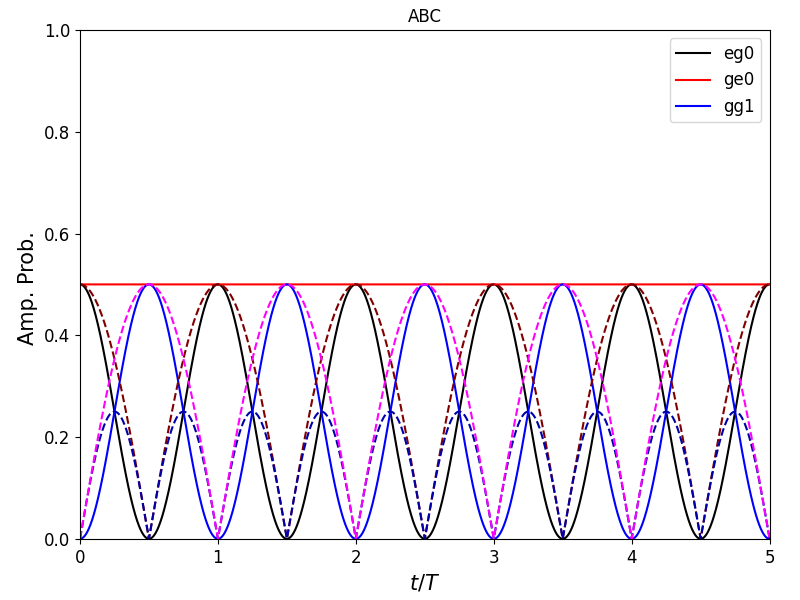
\includegraphics[width=\textwidth]{figuras/ch4/d eg0+ din ABC d=0.png}
        \caption{}
        \label{fig4:dinamica pob eg0 sim resonante}
    \end{subfigure}
    \hfill
    \begin{subfigure}{0.49\textwidth}
        \centering
        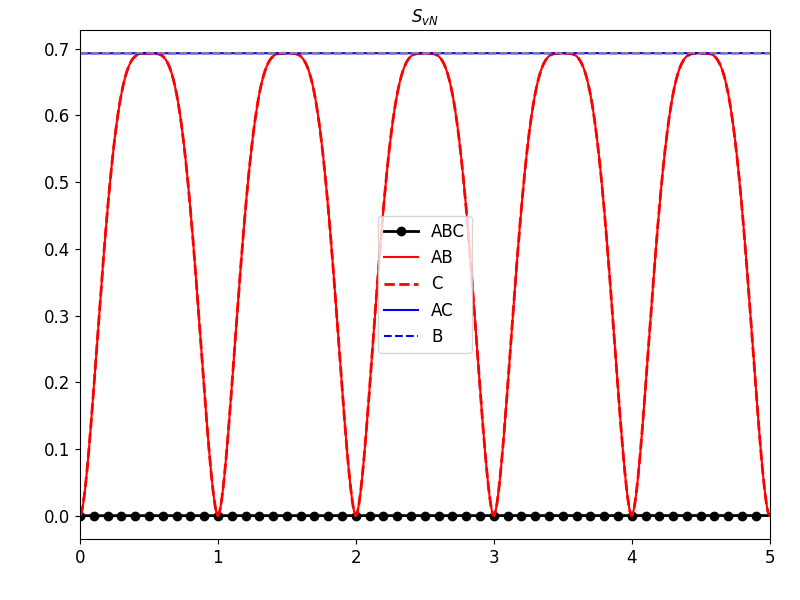
\includegraphics[width=\textwidth]{figuras/ch4/d eg0+ din svn d=0.png}
        \caption{}
        \label{fig4:dinamica svn eg0 sim resonante}
    \end{subfigure}
    \caption{\textcolor{red}{labels, ticks y legens chiquitos. unificar colores}Panel (a):Dinámica poblacional para el caso resonante $\Delta=0$ con el estado inicial entrelazado $\ket{\psi_0}=(\ket{eg0} + \ket{ge0})/\sqrt{2}$. Panel (b):Entropía de von Neuman del sistema total (negro con puntos), y de diferentes subsistemas. En rojo se muestra la entropía del sistema habiendo trazado parcialmente sobre la cavidad, y en azul habiendo trazado parcialmente sobre el átomo B.}
    \label{fig4:dinamica eg0 sim resonante}
\end{figure}

En la figura \ref{fig4:dinamica pob eg0 sim resonante} se muestran las poblaciones y las coherencias correspondientes a la condición inicial $\ket{\psi_0}=(\ket{eg0} + \ket{ge0})/\sqrt{2}$ en el caso resonante, y en la figura \ref{fig4:dinamica svn eg0 sim resonante} se muestra la entropía de Von Neuman, en función del tiempo $t/T$ con $T=2 \pi \Omega(n,j)$  . La entropía de von Neuman es una cantidad que esta definida según:
\begin{equation}\label{eq4:entropia von neuman}
    S=-\Tr(\rho \ln \rho)=-\sum_j \lambda_j \ln \lambda_j
\end{equation}
donde $\rho$ es la matriz densidad del sistema, y $\lambda_j$ son los autovalores de la matriz densidad. La entropía de Von Neuman sirve para determinar si un estado es puro o mixto, ya que $S(\rho)=0$ representa un estado puro, y $S(\rho)=\ln(N)$ representa un estado máximamente mixto, donde $N$ es la dimensión del espacio de Hilbert.
Vemos como el estado $\ket{ge0}$ no evoluciona, ya que en este caso, el átomo B contiene la única excitación y esta aislado. Pero la otra parte, si que evoluciona. Vemos la presencia de las mismas oscilaciones coherentes entre los estados $\ket{eg0}$ y $\ket{gg1}$. La diferencia principal es que en esta caso, el estado de los subsistemas es mixto. Esto se observa claramente en el gráfico de la entropía, pero también se puede deducir este comportamiento desde la figura \ref{fig4:dinamica pob eg0 sim resonante}, ya que a $t/T=0.5$, tenemos el estado $\ket{\psi(T/2)}=\ket{g}_A\otimes(\ket{e_B0_C}+\ket{g_B1_C})/\sqrt{2}$, que es separable solo en el átomo A, y los otros dos están totalmente entrelazados, y por lo tanto al tomar traza parcial tal que el átomo B y la cavidad estén separadas, este estado es máximamente mixto. Vemos como el entrelazamiento entre la cavidad y el átomo B, que están totalmente aislados, evoluciona indirectamente por medio del átomo A, y paradójicamente este queda desentrelazado del sistema para tiempos $t=(k-1/2)T\; ; \; k \in \mathbb{N}$. En este punto notamos algo muy importante, y es que la entropía de von Neuman solo sirve para estados puros. Cuando $t=0$, la entropía del subsistema AB es 0, porque es un estado puro, y esta máximamente entrelazado. Pero al evolucionar, el subsistema AB se hace mixto, y como se observa en la linea azul, la entropía del átomo B es siempre $\log 2$, que según la interpretación de la entropía de von Neuman es que esta siempre máximamente entrelazado. Este no es al caso, y la descripción falla porque el estado AB no es puro.

Entonces, ya que el entrelazamiento es un recurso muy importante y estudiado para las información cuántica, es necesario introducir una medida de entrelazamiento, para poder estudiarlo en este tipo de situaciones. Si bien la entropía de Von Neuman es útil en el caso de estados puros, cuando tenemos estados mixtos como se vio recién, o en el caso de tener un sistema abierto, esta medida ya no sirve. Una de las medidas mas utilizadas y con mayor aplicación es el \textit{Entanglement of Formation} ($E_F$) \cite{an intro to entanglement measures}, que coincide con la entropía de von Neuman para estados puros, y sirve para estados mixtos. El $E_F$ esta definido como
\begin{equation}
    E_F(\rho)=\text{inf}\left( \sum_i p_i E(\ketbra{\psi_i}{\psi_i}) : \rho = \sum_i p_i\ketbra{\psi_i}{\psi_i}\right)
\end{equation}
Esta medida representa el entrelazamiento promedio mínimo entre todas las posibles descomposiciones puras de $\rho$, donde $E(\ketbra{\psi_i}{\psi_i})=S(\tr_B{\ketbra{\psi_i}{\psi_i}})$ es la entropía de von Neuman, que es la medida que se utiliza para estados puros. Esta definición es general, pero en el caso presente, nos sirve una simplificación de esta medida que se obtiene si se estudia el entrelazamiento entre dos qu-bits, como lo son los átomos A y B. Esta medida es la concurrencia, y esta definida como
\begin{equation}
    C(\rho)=\text{max}\{0,\lambda_1-\lambda_2-\lambda_3-\lambda_4\}
\end{equation}
donde los $\lambda_i$ son las raíces de los autovalores, en orden decreciente, de la matriz $\rho\sigma_y\otimes\sigma_y\rho^*\sigma_y\otimes\sigma_y$, donde $\rho*$ es el conjugado (sin transponer) de $\rho$. La concurrencia y la entropía de formación $E_F$ están relacionadas, y la concurrencia obtiene su interpretación a través de esta. Un estado máximamente entrelazado tiene $C(\rho)=1$ y un estado separable $C(\rho)=0$. 


\begin{figure}[H]
    \begin{minipage}[c]{0.67\textwidth}
        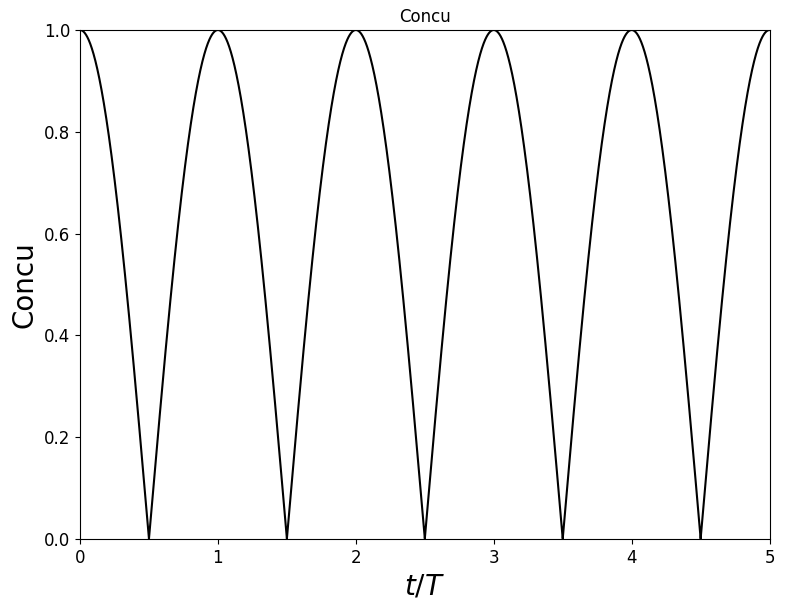
\includegraphics[width=\textwidth]{figuras/ch4/d eg0+ concu d=0.png}
    \end{minipage}\hfill
    \begin{minipage}[c]{0.3\textwidth}
    \caption{Concurrencia en el caso resonante para estado inicial $\ket{eg0}+\ket{ge0}$
         } \label{fig4:concu eg0 sim}
  \end{minipage}
\end{figure}
En la figura \ref{fig4:concu eg0 sim} se observa la concurrencia entre los átomos AB, para el caso estudiado anteriormente. Como era de esperar, a $t=0$ el estado es máximamente entrelazado, y luego el entrelazamiento se pierde a $t=T/2$, donde el átomo B esta entrelazada con la cavidad. 

\subsection{Interacción átomo-átomo}

El siguiente paso es analizar el rol de las interacciones entre los átomos, aun manteniendo el apantallamiento $\alpha=0$. Para esto, se sigue utilizando las mismas condiciones iniciales y el átomo B seguirá sin interactuar con la cavidad, pero se considera ahora que la interacción entre átomos dadas por los parámetros $k$ y $J$ ahora serán distintos de cero. Para comenzar, en la figura \ref{fig4:k eg0 abc} se observa la evolución temporal para el estado inicial $\ket{\psi_0}=\ket{eg0}$, con $\Delta = 0$, $J=0$ pero $k=0.1g$. Recordemos que $k$ es la intensidad de la interacción $\sigma^{(1)}_+\sigma^{(2)}_-+\text{c.c.}$ (ver \ref{eq4:H}).

\begin{figure}[h]
    \begin{minipage}[c]{0.67\textwidth}
        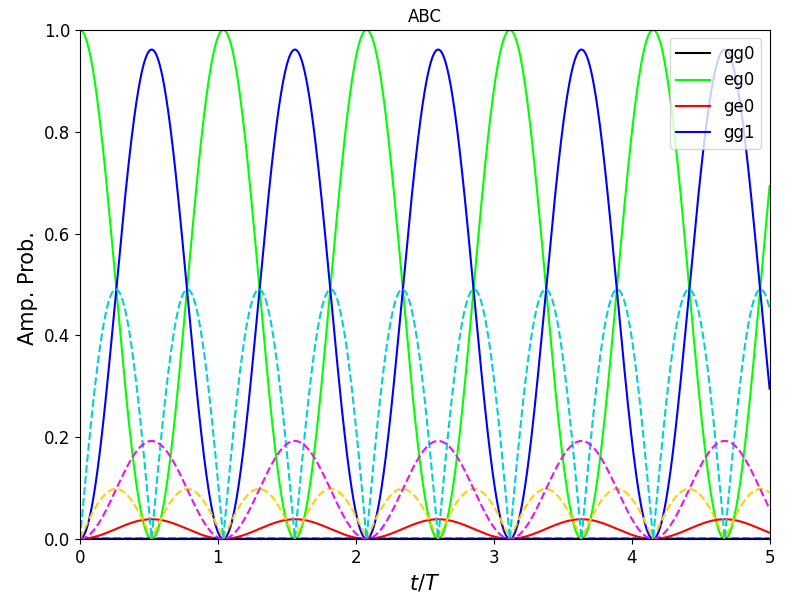
\includegraphics[width=\textwidth]{figuras/ch4/k eg0 ABC.png}
    \end{minipage}\hfill
    \begin{minipage}[c]{0.3\textwidth}
    \caption{Dinámica poblacional para la condición inicial $\ket{\psi_0}=\ket{eg0}$, para los parámetros $\Delta=0$, $J=0$ y $k=0.1g$. Las lineas solidas se corresponden con las poblaciones de la matriz densidad total del sistema; en azul la probabilidad de encontrar al estado en el estado $\ket{gg1}$, en verde en $\ket{eg0}$, en rojo $\ket{ge0}$, y en negro $\ket{gg0}$. Las lineas rayadas son las coherencias entre estas poblaciones, la violeta entre $\ket{gg1}$ y $\ket{ge0}$, la celeste entre $\ket{eg0}$ y $\ket{gg1}$ y la amarilla entre $\ket{eg0}$ y $\ket{gg1}$.
         } \label{fig4:k eg0 abc}
  \end{minipage}
\end{figure}
Lo que sucede es que la excitación esta inicialmente en el átomo A, y como siempre, se observan oscilaciones entre los estados $\ket{eg0}$ y $\ket{gg1}$, la diferencia es que al haber interacciones entre los átomos, ahora la excitación inicial que esta en el átomo A, sufre dos procesos diferentes, primero la oscilación, y ademas, la interacción con el átomo B. Al tener la excitación el átomo A, una parte de esta se va hacia la cavidad, y la otra hacia el átomo B, excitándolo parcialmente. La amplitud de la oscilación depende de la intensidad de la interacción $k$. Si nos concentramos en la curva roja, vemos que su pendiente crece mientras que la probabilidad de $\ket{eg0}$ es mayor a la de $\ket{gg1}$, luego la amplitud crece, pero de manera desacelerada, hasta que la probabilidad del estado $\ket{eg0}$ es nula. En ese momento, ya no hay excitación que pasar del átomo A al B, y el proceso se revierte. Antes de analizar el entrelazamiento entre los átomos, se observa en la figura \ref{fig4:k eg0 sim abc} la dinámica para los mismos parámetros, pero para la condición inicial entrelazada $\ket{\psi_0}=(\ket{eg0}+\ket{ge0})/\sqrt{2}$:
\begin{figure}[h]
    \begin{minipage}[c]{0.67\textwidth}
        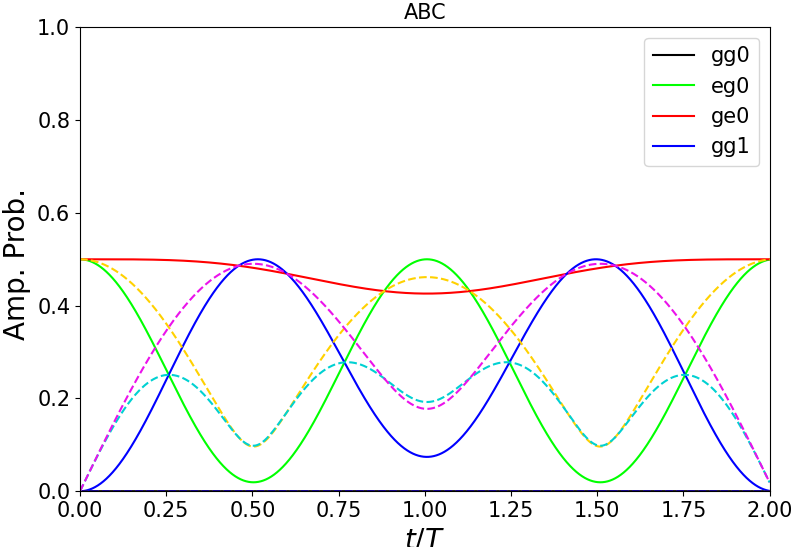
\includegraphics[width=\textwidth]{figuras/ch4/k eg0+ ABC.png}
    \end{minipage}\hfill
    \begin{minipage}[c]{0.3\textwidth}
    \caption{Dinámica poblacional para la condición inicial $\ket{\psi_0}=\ket{eg0+ge0}$, para los parámetros $\Delta=0$, $J=0$ y $k=0.1g$. Las coherencias y poblaciones tienen los mismos colores que la figura anterior \ref{fig4:k eg0 abc}
         } \label{fig4:k eg0 sim abc}
  \end{minipage}
\end{figure}
La dinámica en este caso presenta oscilaciones en la población de $\ket{ge0}$ con un periodo dos veces mas grande. Esto se debe a una \"pelea\" entre los estados $\ket{eg0}$ y $\ket{ge0}$, ya que tienen las excitaciones en diferentes átomos. Inicialmente, como los estados están entrelazados, no esta bien definido en cual de los dos átomos esta la excitación, entonces la interacción $k$ se anula y vemos que tiene pendiente 0. Entonces la dinámica inicial es igual que para $k=0$ y comienza a oscilar. Apenas baja la curva verde, la probabilidad de encontrar la excitación en el átomo B es mayor que la del átomo A, entonces lo que sucede es que el átomo B comienza a perder esta excitación y se la da lentamente al átomo A, y por lo tanto la oscilación del estado $\ket{eg0}$ no llega a tener amplitud nula en $t/T=0.5$. Luego, la evolución sigue su curso oscilante, y al llegar a $t=T$, vemos que la probabilidad de encontrar la excitación en el átomo A es mayor, y por lo tanto comienza a revertirse la situación, hasta completar el ciclo para $t=2T$. \textcolor{red}{no es exacto pq puse algo mal en el codigo, pero ahora esta corregido y da bien. tengo que cambiar estas imagenes.} 

El entrelazamiento entre los atomos se analiza utilizando la concurrencia, como se muestra en la figura \ref{fig4:concu k}, donde \ref{fig4:concu k eg0} muestra la condicion inicial separable $\ket{eg0}$, y \ref{fig4:concu k eg0 sim} el entrelazamiento para la condicion inicial entrelazada $\ket{eg0+ge0}$. 
\begin{figure}[h]
    \centering
    \begin{subfigure}{0.49\textwidth}
        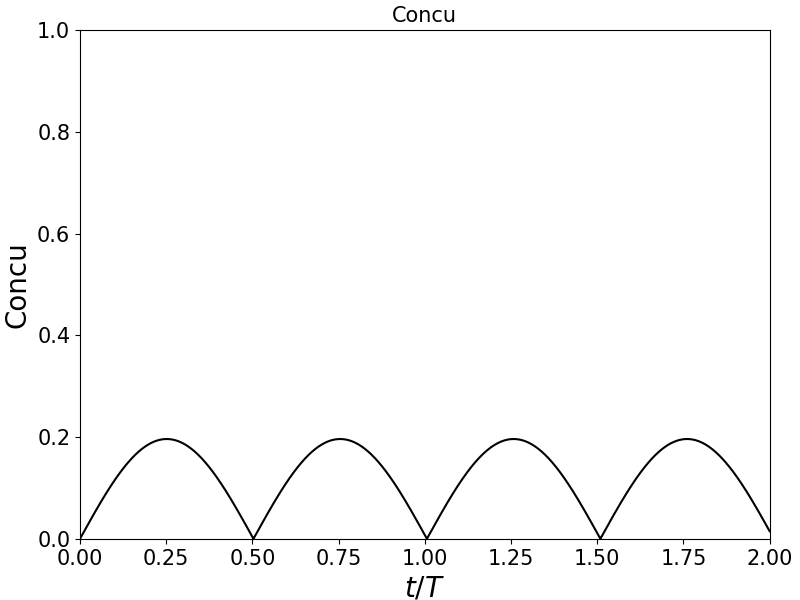
\includegraphics[width=\textwidth]{figuras/ch4/k eg0 concu.png}
        \caption{$\ket{eg0}$}
        \label{fig4:concu k eg0}
    \end{subfigure}
    \hfill
    \begin{subfigure}{0.49\textwidth}
        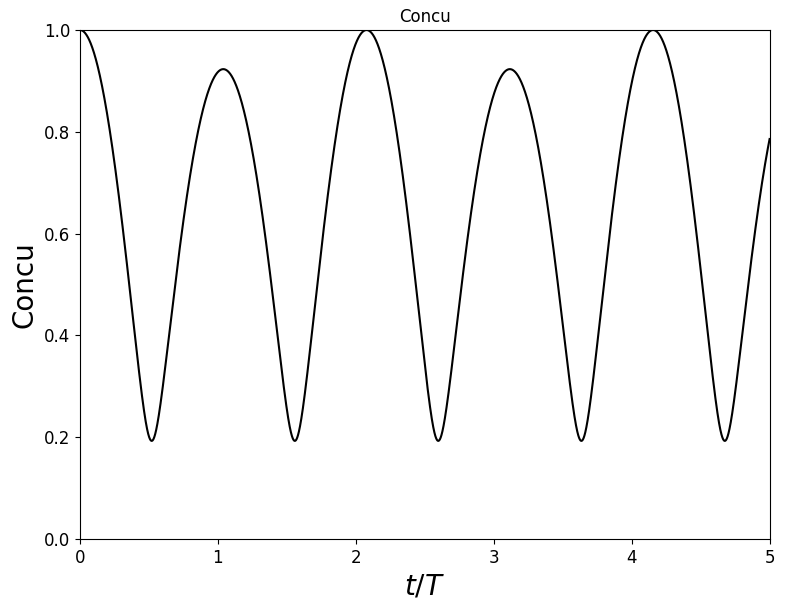
\includegraphics[width=\textwidth]{figuras/ch4/k eg0+ concu.png}
        \caption{$\ket{eg0+ge0}$}
        \label{fig4:concu k eg0 sim}
    \end{subfigure}
    \caption{\textcolor{red}{rehacer por labels chiquitos}Dinamica de entrelazamiento para $\Delta=0$, $J=0$ y $k=0.1g$}
    \label{fig4:concu k}
\end{figure}

Ahora vamos a ver $k=0$ y $J\neq 0$. En la figura \ref{fig4:j alpha0}, vemos que, si bien la dinamica es similar, los atomos no se entrelazan.

\begin{figure}[H]
    \centering
    \begin{subfigure}{0.49\textwidth}
        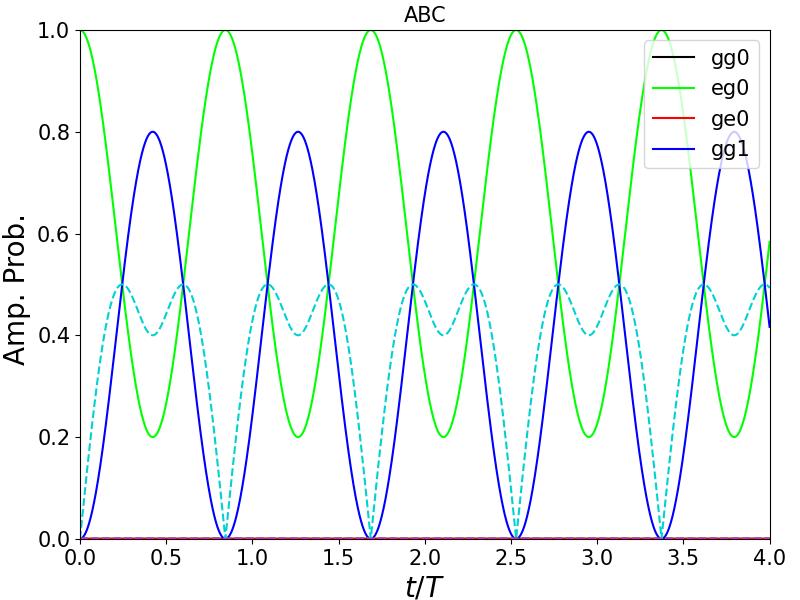
\includegraphics[width=\textwidth]{figuras/ch4/j eg0 abc.png}
        \caption{$\ket{eg0}$ Poblaciones}
        \label{fig4:pob j eg0}
    \end{subfigure}
    \hfill
    \begin{subfigure}{0.49\textwidth}
        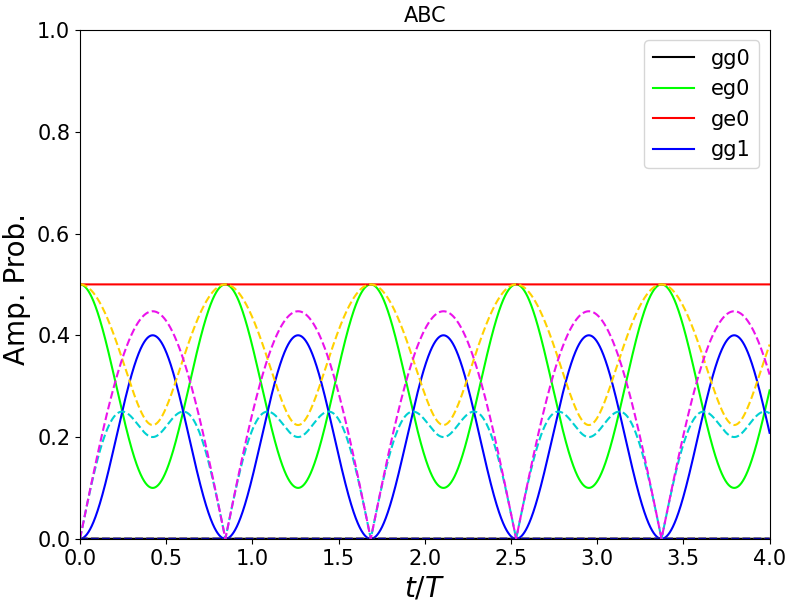
\includegraphics[width=\textwidth]{figuras/ch4/j eg0+ge0 abc.png}
        \caption{$\ket{eg0+ge0}$ Poblaciones}
        \label{fig4:pob j eg0 sim}
    \end{subfigure}
    \vfill
    \begin{subfigure}{0.49\textwidth}
        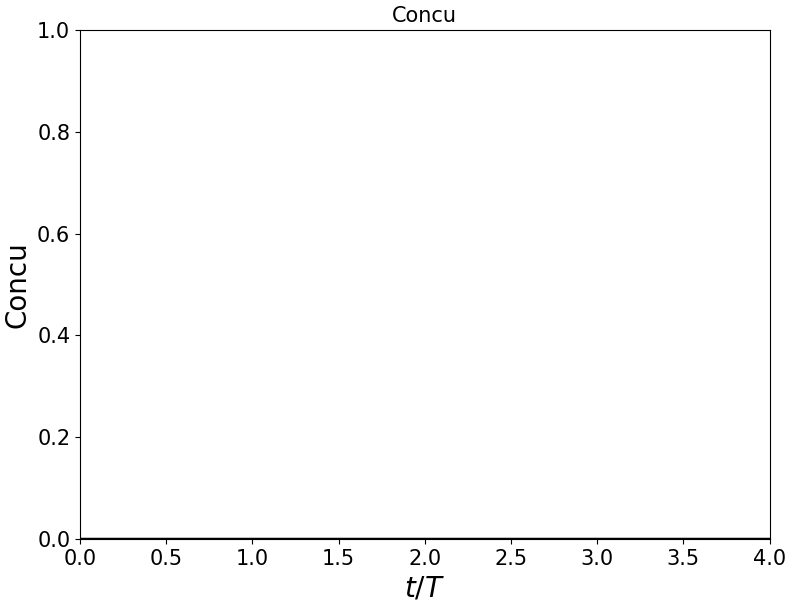
\includegraphics[width=\textwidth]{figuras/ch4/j eg0 concu.png}
        \caption{$\ket{eg0}$ Concurrencia}
        \label{fig4:pob j eg0}
    \end{subfigure}
    \hfill
    \begin{subfigure}{0.49\textwidth}
        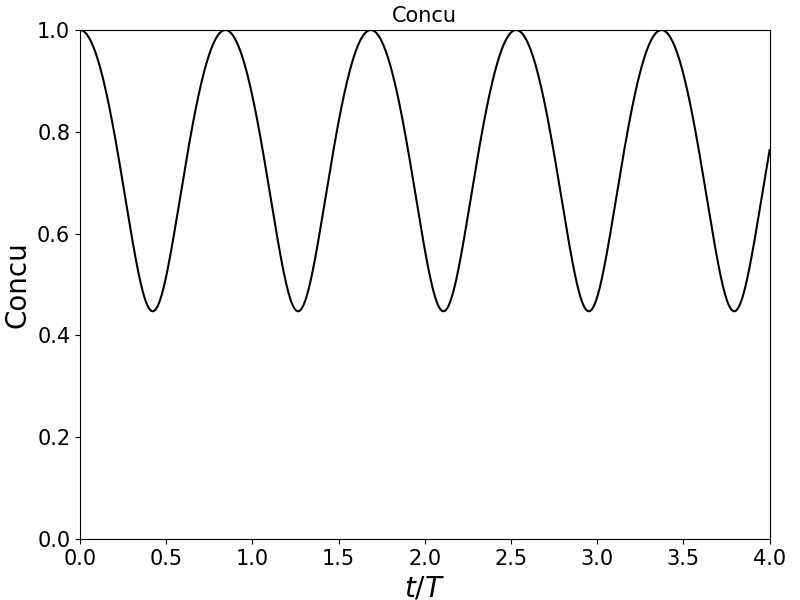
\includegraphics[width=\textwidth]{figuras/ch4/j eg0+ge0 concu.png}
        \caption{$\ket{eg0+ge0}$ Concurrencia}
        \label{fig4:pob j eg0 sim}
    \end{subfigure}
    \caption{$\Delta=0$, $J=0.5g$ y $k=0$}
    \label{fig4:j alpha0}
\end{figure}
Vemos que la diferencia prinipal entre la interaccion tipo Isign ($J\sigma_z^{(1)}\sigma_z^{(2)}$) y la dipolar ($k\sigma_+^{(1)}\sigma_-^{(2)}+\text{c.c.}$), es que el segundo parece entrelazar los atomos, ya que en el primer caso, el efecto es separar los niveles de energia, pero en el segundo no solo eso, sino que tambien pasa excitaciones de un atomo al otro. Si bien esto nos sirve para entender intuitivamente el efecto, el problema de este analisis es que estamos asumiendo cosas no fisicas mediante el apantallamiento y la asimetria que imponemos entre los dos atomos. Esto, lleva a estos analisis que en realidad no son correctos, ya que si miramos el Hamiltoniano del sistema sin apantallamiento \ref{eq4:H}, donde usamos la base con estados simetricos y antisimetricos \ref{ec4:base}, el efecto de ambos parametros deberia ser el mismo, ya que solo aparecen en la diagonal principal. Si bien la interaccion $J$ actua sobre todos los estados, y el $k$ solamente solo sobre los $\ket{egn\pm gen}$, su principal funcion es separar las energias de los estados de la base.
Entonces sera necesario retomar este analisis sin apantallamiento y con la base \ref{ec4:base}.
\subsection{Medio Kerr}

Ahora nos concentramos en el efecto del medio Kerr. Para esto, apagamos las interacciones interatomicas $k=J=0$, y ahora se modifica el medio a traves del parametro $\chi$. 
\begin{figure}[h]
    \centering
    \begin{subfigure}{0.49\textwidth}
        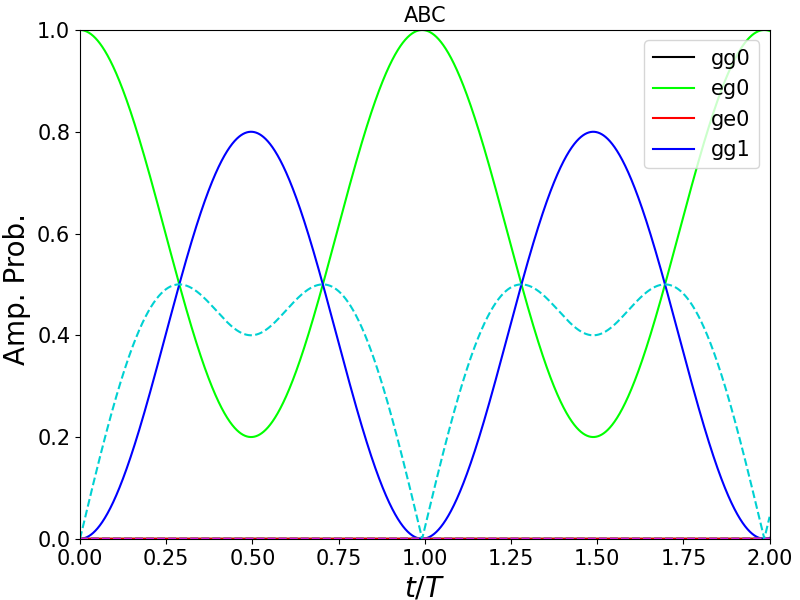
\includegraphics[width=\textwidth]{figuras/ch4/x eg0 abc.png}
        \caption{$\ket{eg0}$}
        \label{fig4:pob x eg0}
    \end{subfigure}
    \hfill
    \begin{subfigure}{0.49\textwidth}
        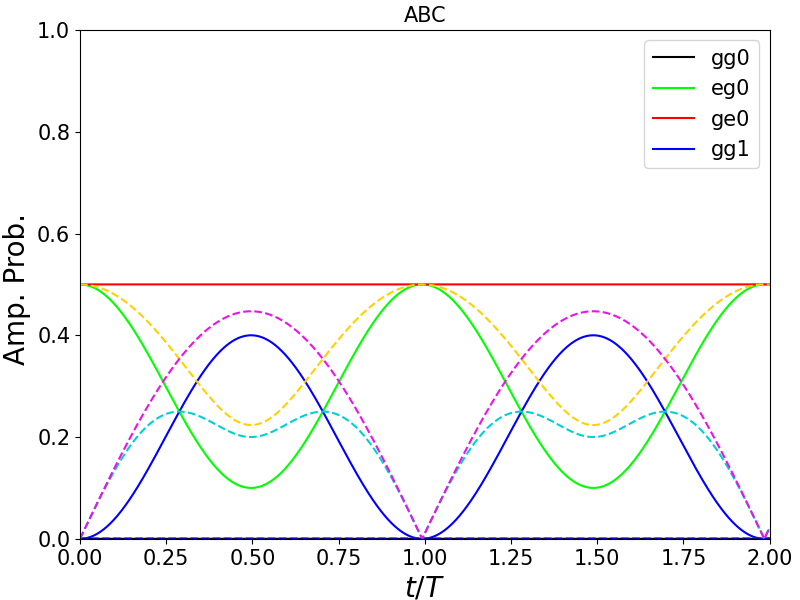
\includegraphics[width=\textwidth]{figuras/ch4/x eg0+ abc.png}
        \caption{$\ket{eg0+ge0}$}
        \label{fig4:pob x eg0 sim}
    \end{subfigure}
    \caption{Dinamica de poblaciones para $x=g$}
    \label{fig4:pob x}
\end{figure}

Al igual que en el caso de 1 atomo, se puede observar en las ecuaciones \ref{ec4:autoenergias} y \ref{ec4:parametros solucion}, la frecuencia depende del medio. En la figura \ref{fig4:pob x} el tiempo esta normalizado con la frecuencia, entonces no se nota el cambio. Pero lo que es necesario analizar, es como las oscilaciones no son totalmente coherentes, en el sentido de que la probabilidad del estado $\ket{gg1}$ nunca alcanza la amplitud inicial de la oscilacion, como en el caso de $\chi=0$. Esto se debe a que el aumento de $\chi$ hace que las energias de ambos estados se separen, y por lo tanto hace que las transiciones entre los estados sea menos probable. Este comportamiento tambien se observa si el estado inicial se toma como $\ket{gg1}$. Es logico estudiar el entrelazamiento en este caso. En la figura \ref{fig4:concu x} se muestran las concurrencias para ambas condiciones iniciales. Es interesante comparar la figura \ref{fig4:concu x eg0 sim} con la figura en el caso de $\chi=0$ para esta misma condicion inicial, la figura \ref{fig4:concu eg0 sim}. En principio se puede pensar que el medio no lineal rompe con el entrelazamiento del sistema, pero como se ve al comparar estas figuras, la interpretacion correcta es que el medio no hace mas que alentizar el comportamiento preexistente de la cavidad, ya que en este caso, no destruye el entrelazamiento, sino que lo conserva por virtud de haber realentizado las amplitudes de oscilacion entre los dos estados dinamicos.
\begin{figure}[h]
    \centering
    \begin{subfigure}{0.49\textwidth}
        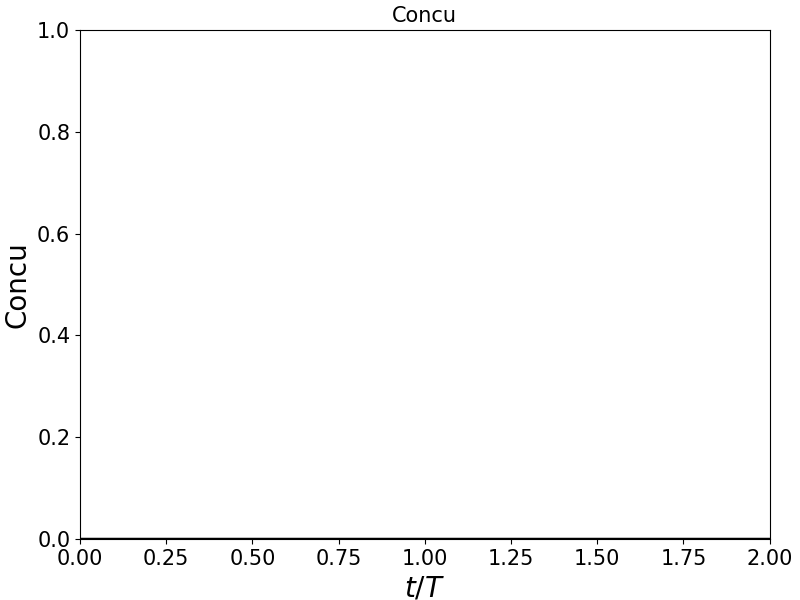
\includegraphics[width=\textwidth]{figuras/ch4/x eg0 concu.png}
        \caption{$\ket{eg0}$}
        \label{fig4:concu x eg0}
    \end{subfigure}
    \hfill
    \begin{subfigure}{0.49\textwidth}
        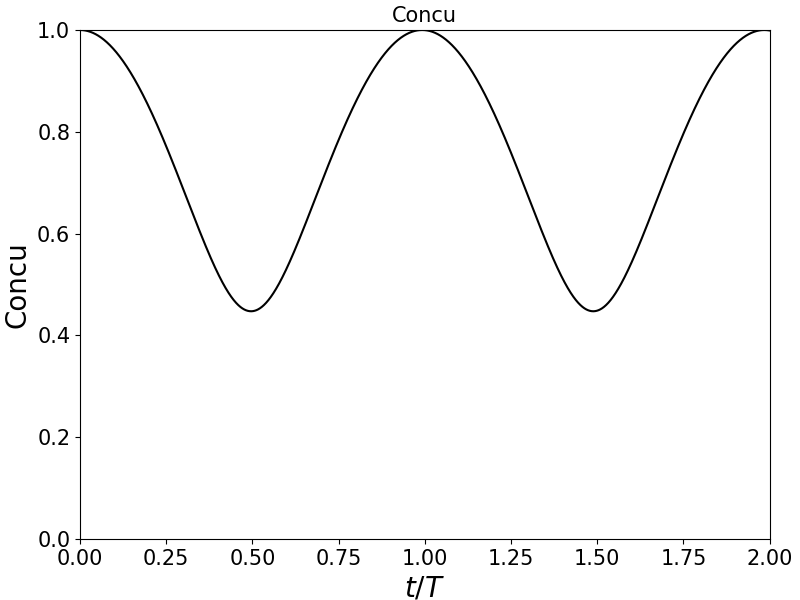
\includegraphics[width=\textwidth]{figuras/ch4/x eg0+ concu.png}
        \caption{$\ket{eg0+ge0}$}
        \label{fig4:concu x eg0 sim}
    \end{subfigure}
    \caption{Dinamica de entrelazamiento para $x=g$}
    \label{fig4:concu x}
\end{figure}
Tambien se puede intentar de recuperar el comportamiento visto en el modelo de 1 atomo, que el medio Kerr no es mas que un desplazamiento lateral en las frecuencias, ademas de modificar las amplitudes. Para esto se realiza otra evolucion para $\chi=\Delta=\frac{g}{2}$, y se compara con el caso en que $\chi=\Delta=0$
\begin{figure}[h]
    \centering
    \begin{subfigure}{0.49\textwidth}
        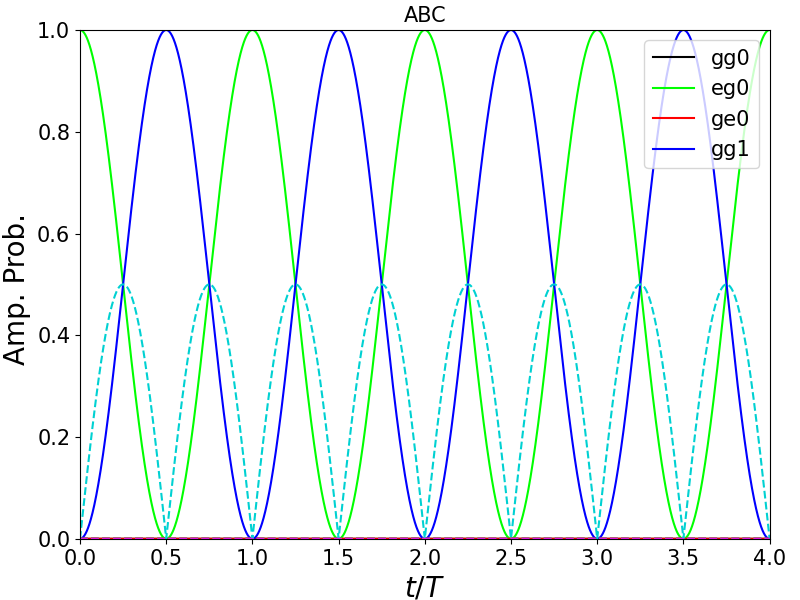
\includegraphics[width=\textwidth]{figuras/ch4/d=x=0 eg0 abc.png}
        \caption{$\Delta=\chi=0$}
        \label{fig4:comparacion kerr pob 1}
    \end{subfigure}
    \hfill
    \begin{subfigure}{0.49\textwidth}
        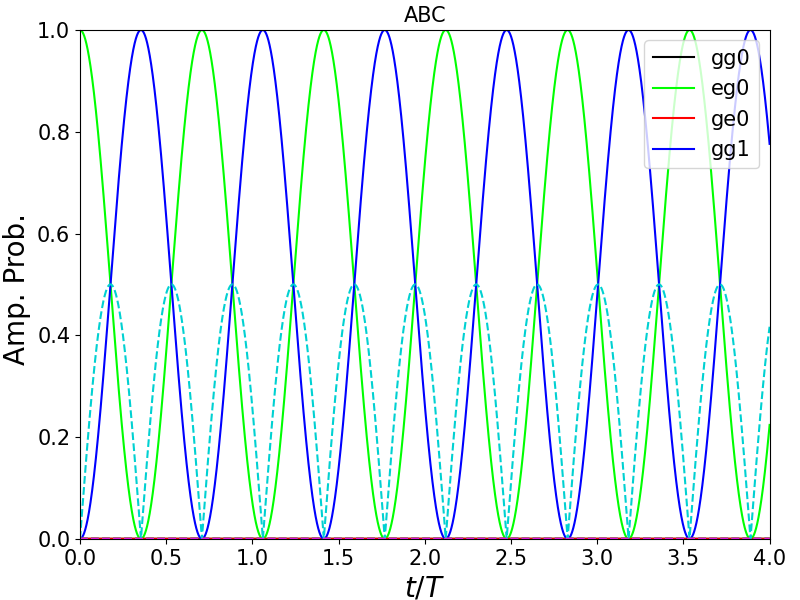
\includegraphics[width=\textwidth]{figuras/ch4/d=x=0.5 eg0 abc.png}
        \caption{$\Delta=\chi=0.5g$}
        \label{fig4:comparacion ker pob 2}
    \end{subfigure}
    \caption{Dinamica de entrelazamiento para $x=g$}
    \label{fig4:comparacion d vs x}
\end{figure}
Vemos como se anula el efecto del medio, y la dinamica es la misma pero con un cambio en la frecuencia. Al igual que antes, aumenta la frecuencia

\subsection{Batidos}

Al complejizar el problema, comienzan a aparecer batidos, comportamiento que se atribuye a la modulacion de dos procesos simultaneos. Por ejemplo, si observamos la evolucion temporal con $\chi\neq0$ y $k\neq0$, entonces el primero disminuye la amplitud de oscilacion de, los estados con mayor cantidad de fotones en la cavidad, que dentro del subespacio $N$ la jerarquia del medio sera favorecer a los estados $\ket{eg,N-1}$ y $\ket{ge,N-1}$ por sobre el $\ket{ggN}$. Por el contrario, se observo que en esta situacion, el termino de interaccion entre los atomos disminuye la amplitud del estado $\ket{ggN}$ como se vio en la seccion anterior. Por lo tanto, si tenemos dos procesos que estan en juego y sus efectos son similares, entonces es esperable que se observen oscilaciones moduladas. No vale la pena mostrar la dinamica de las poblaciones, porque no se pueden sacar conclusiones muy importantes, pero si podemos observar la trayectoria en la esfera de bloch, para dar una idea de la complejidad de la evolucion.

\section{Dinamica sin apantallamiento}

Al sacar el apantallamiento, es necesario utilizar la base mencionada anteriormente \ref{ec4:base}, ya que los atomos son indistinguibles y esta base es mas apropiada. Ademas, el Hamiltoniano desacopla los estados antisimetricos, facilitando la solucion. Por lo tanto, se procede a estudiar la dinamica sacando el apantallamiento. Lo que nos interesa estudiar es el entrelazamiento entre las diferentes partes del sistema, y su dependencia con los parametros. 

\subsection{Dinamica con disipacion}

Lo primero que hay que mirar es la dependencia de la dinamica con el regimen de acoplamiento, esperamos un comportamiento igual al del caso de un atomo \ref{sec3:regimen acoplamiento}. Recordemos que el regimen de acoplamiento fuerte (SC) es el caso en donde la interaccion entre cavidad y atomos es mayor a la interaccion entre sistema y entorno.
\begin{figure}[h]
    \centering
    \begin{subfigure}{0.7\textwidth}
        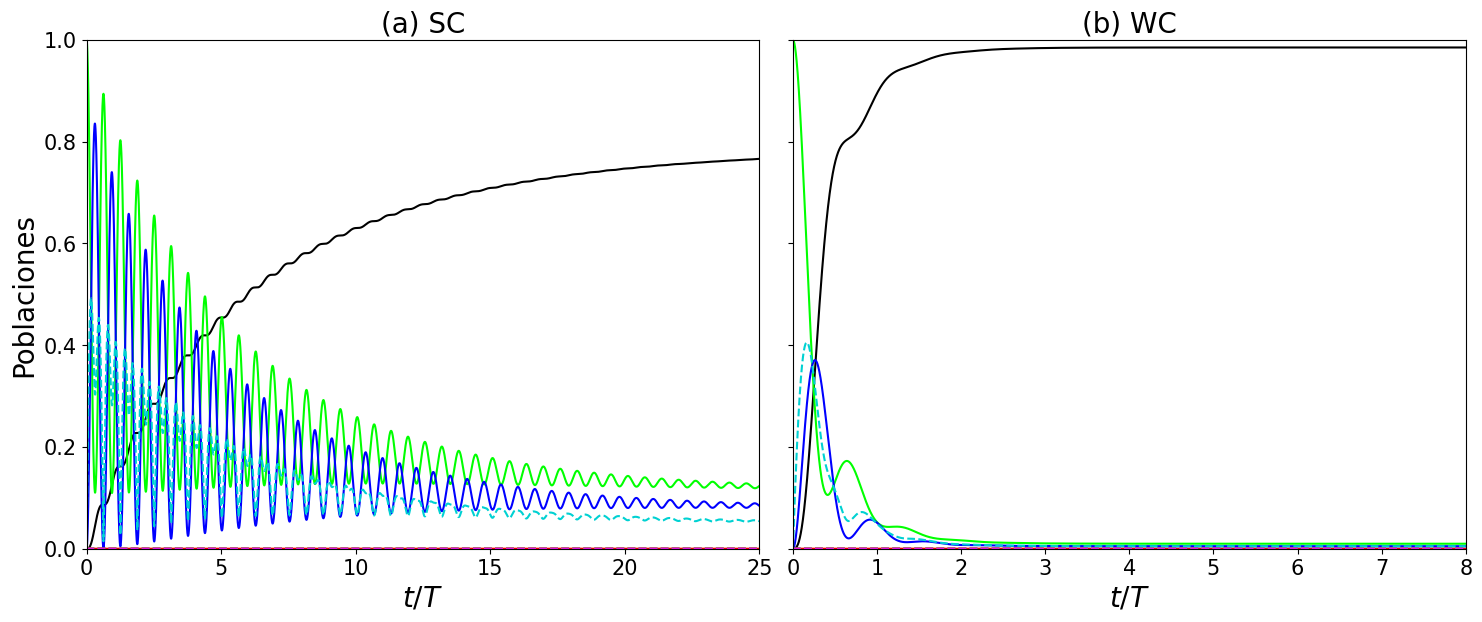
\includegraphics[width=\textwidth]{figuras/ch4/sc vs wc eg0 sim j0.5.png}
        \caption{$\ket{eg0+ge0}$. $\Delta=\chi=k=0$, $J=0.5g$}
        \label{fig4:acoplamiento eg0 sim}
    \end{subfigure}
    \vfill
    \begin{subfigure}{0.7\textwidth}
        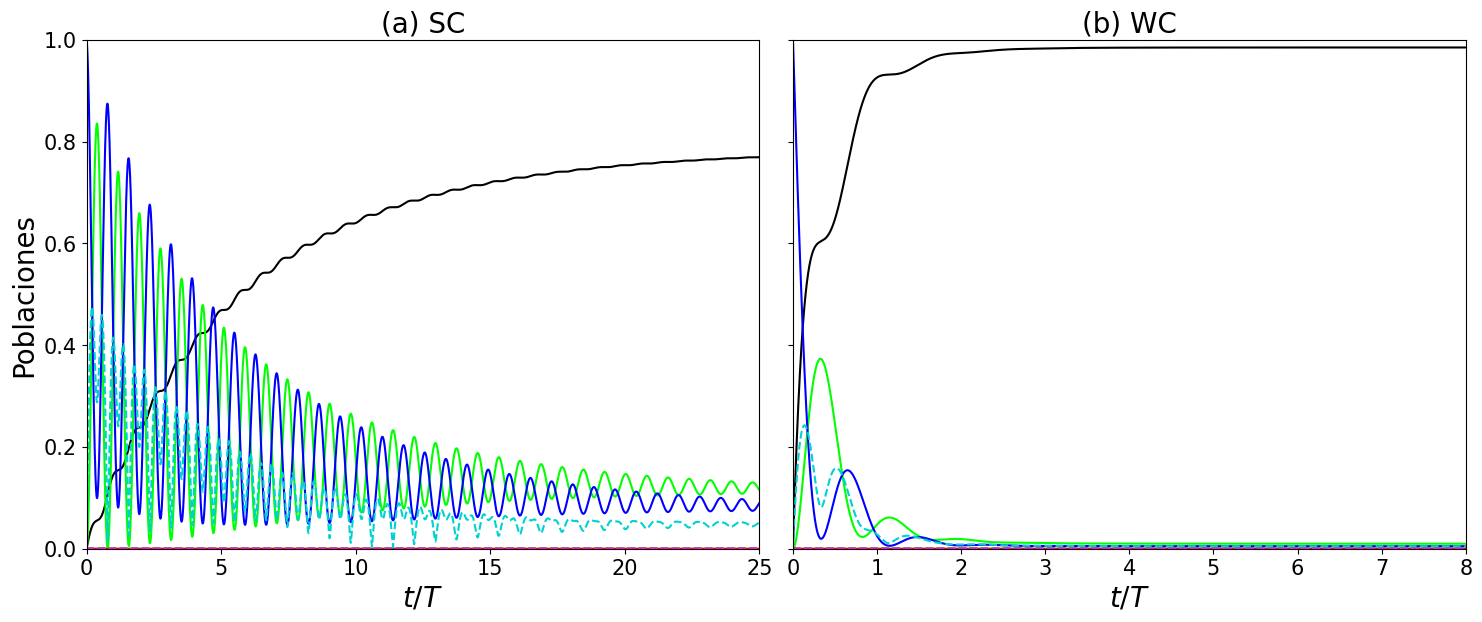
\includegraphics[width=\textwidth]{figuras/ch4/sc vs wc gg1 k=0.5.png}
        \caption{$\ket{gg1}$. $\Delta=\chi=J=0$, $k=0.5g$ }
        \label{fig4:acoplamiento gg1}
    \end{subfigure}
    \caption{Dependencia de las poblaciones con el regimen de acoplamiento, para $\Delta=J=\chi=0$ y $k=0.5g$, y para dos condiciones iniciales diferentes.}
    \label{fig4:regimen acoplamiento}
\end{figure}
En  la figura \ref{fig4:regimen acoplamiento} se  muestran las coherencias y las poblaciones, como se esperaba, estas tienen el mismo comportamiento que en el caso de 1 atomo. Notablemente, se puede ver el efecto de la interaccion entre los atomos, como se separan las energias inicialmente las oscilaciones no logran la inversion total de poblacion, solo una inversion parcial, y a tiempo largos la disipacion hace que se tenga una mayor probabilidad de encontrar al sistema en el estado $\ket{eg0+ge0}$ ya que tiene menor energia. Eventualmente alcanza su estado estacionario. Lo que se recupera, ahora que ya no hay apantallamiento, es que ambos tipos de interaccion ($J$ y $k$) generan entrelazamiento. Como es de esperarse, en ambos casos la concurrencia es oscilatoria por la naturaleza oscilante del problema, pero ahora, como el estado al que oscila

Nuevamente, nos concentraremos en el regimen SC. Si bien hasta ahora nos concentramos en estados con 1 excitacion, y es interesante por sus implicancias y similitudes al oedelo de 1 atomo, considerar estados con mayor cantidad de excitaciones hace a la riqueza del problema. Si solo consideranos $N=1$, tenemos 3 estados en el subespacio, de los cuales uno es el estado antisimetrico $\ket{eg0-ge0}$, que esta desconectado de los otros estados, y por lo tanto efectivametne se tiene un modelo de Jaynes-Cummings normal. Si vamos a $N=2$, ahora tenemos 4 estados en el subespacio, y 3 son relevantes. Por lo tanto, ahora veremos cuales son los efectos de las interacciones y la dinamica para estados iniciales en el subespacio de $N=2$. Para mantener el paralelismo, comenzaremos con el estado $\ket{eg1+ge1}$, pero como se vera, las condiciones iniciales cambian totalmente la dinamica de entrelazamiento del sistema. La enorme cantidad de posibilidades para elegir condiciones iniciales, hace que estudiar todos sea imposible, asi que nos concentraremos en algunos.
Al tener 3 estados dinamicamente relevantes, tenemos 3 autoestados con sus respectivas autoenergias, y por lo tanto tenemos 3 frecuencias que compiten entre si, y son las 3 frecuencias de Rabi del sistema:
\begin{equation}
    \begin{aligned}
        \Omega^{(n)}_{12} &= E^{(n)}_2-E^{(n)}_1 \\
        \Omega^{(n)}_{23} &=E^{(n)}_3-E^{(n)}_2 \\
        \Omega^{(n)}_{31} &= E^{(n)}_1-E^{(n)}_3         
    \end{aligned}
    \label{ec4:frecuencias de rabi}
\end{equation}
Estas frecuencias se muestran en funcion del detunning $\Delta$ y para diferentes valores de $\chi$ y de $k-J$ en la figura \ref{fig4:frecuencias de rabi}.
\begin{figure}
    \centering
    \begin{subfigure}{\textwidth}
        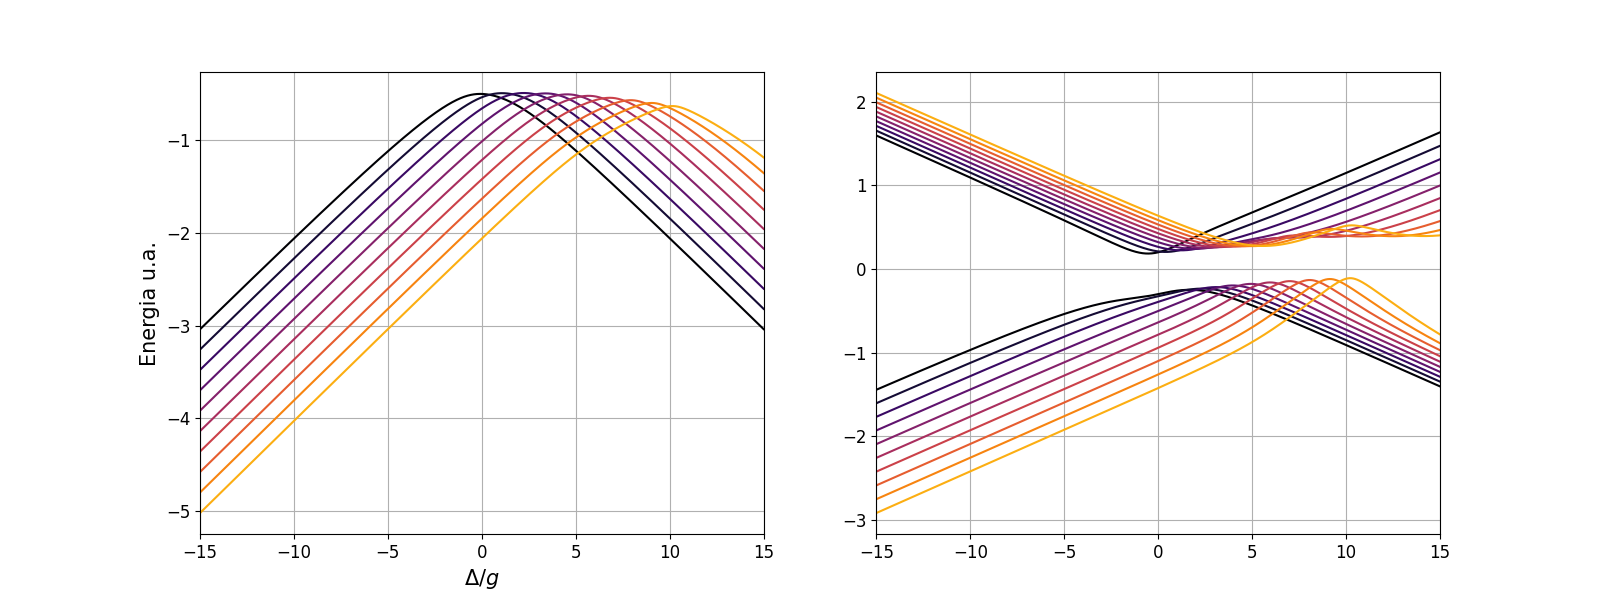
\includegraphics[width=\textwidth]{figuras/ch4/frecuencias k=0.5g chilist.png}
        \caption{Frecuencias de Rabi en funcion del detunning, para diferentes valores de $\chi/g\in[0,5]$ y $k-J=0.5g$. A la izquierda $\Omega_{12}$ y a la derecha $\Omega_{23}$ y $\Omega_{13}$}
        \label{fig4:rabi chi}
    \end{subfigure}
    \vfill
    \begin{subfigure}{\textwidth}
        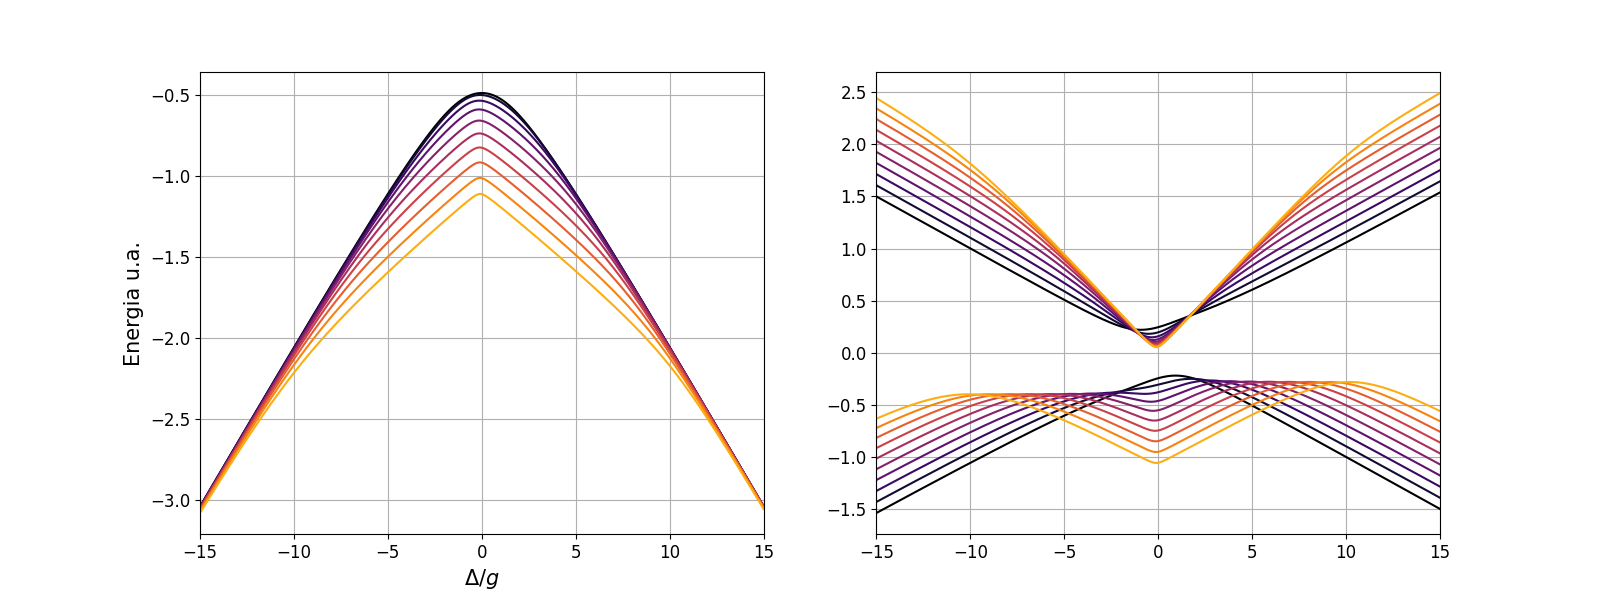
\includegraphics[width=\textwidth]{figuras/ch4/frecuencias x=0 klist.png}
        \caption{Frecuencias de Rabi en funcion del detunning, para diferentes valores de $k-J\in[0,5g]$ y $\chi=0$. A la izquierda $\Omega_{12}$ y a la derecha $\Omega_{23}$ y $\Omega_{13}$. Solo se muestra una de las ramas.}
        \label{fig4:rabi k}
    \end{subfigure}
    \caption{Frecuencias de Rabi en funcion del detunning $\Delta$ para diferentes valores de $\chi$, y $|k-J|$, donde las frecuencias de Rabi son $\Omega^{(2)}_{ij}=E^{(2)}_{j}-E^{(2)}_{i}$}
    \label{fig4:frecuencias de rabi}
\end{figure}
En esta solo se muestra una de las dos ramas (se puede tener $\pm \Omega_{ij}$) por simplicidad. Lo que podemos concluir de esto es que la frecuencia $\Omega^(2)_{12}$ se comporta de manera similar a la frecuencia de Rabi del JC de 1 atomo, que es tambien igual a la $\Omega^(1)$; en ambos casos la diferencia de energia presenta un maximo que se desplaza lateralmente al aumentar el parametro $\chi$, pero presenta una sutil diferencia ya que tambien el maximo aumenta en valor absoluto. Tambien se observa en la figura \ref{fig4:rabi k}, a la izquierda, como depende esta frecuencia al aumentar $k-J$, y vemos que el maximo ya no se desplaza lateralmente, sino que solo aumenta en valor absoluto. Por otro lado, en los paneles derechos, se puede analizar que sucede con las frecuencias al aumentar $\chi$ (fig. \ref{fig4:rabi chi}) y $k-J$ (fig. \ref{fig4:rabi k}). Es interesante ver como al aumentar $\chi$, se comienza a observar un maximo y minimo local para la frecuencia $\Omega^{(2)}_{23}$ (la superior). Similarmente, pero en la rama superior, se observa este mismo comportamiento al aumentar $k-J$.

La dinamica para el caso de $N\geq2$ es muy complicada, ya que ahora se tienen 3 frecuencias diferentes, y predecir que sucede para cada combinacion de parametros y para cada condicion inicial se hace muy complicado, por lo tanto, el analisis para estos casos no puede ser muy profundo. Lo que se puede distinguir es que cuando $\chi,k-J>g$, se comienzan a observar estos minimos y maximos locales en las frecuencias, y se puede intentar de ver cual es el efecto que tiene esto en el entrelazamiento de los atomos, y tambien se puede observar si hay alguna relacion entre los parametros, por ejemplo como se encontro para el caso de 1 atomo (y para el subespacio de N=1) que hay una clara relacion entre el detunning $\Delta$ y el medio $\chi$.
\section{Dinamica de entrelazamiento}
Para estudiar la dinamica de entrelazamiento entre los dos atomos, nos centraremos en la concurrencia ($0\leq C_{AB} \leq 1$).
En primer lugar consideraremos una cavidad lineal, y finalmente veremos cual es el efecto del medio Kerr sobre el entrelazamiento.

\subsection{Cavidad lineal}
Lo primero que tenemos que analizar es los efectos de las interacciones entre los atomos, como ya vimos,  vamos a definir dos regimenes, que llamaremos Strong Interacting (SI) y Weak Interacting (WI), refiriendonos a la interaccion entre los atomos con respecto a la cavidad. El SI sera cuando la interaccion entre los atomos es fuerte en comparacion con la cavidad, es decir $k-J>g$, y WI con $k,J<g$. Ya que no se definio un limite muy claro, trabajaremos con un valor representativo de cada regimen, $k-J=0.1g$ y $k-J=5g$ respectivamente. Para ilustrar la las diferencias entre condiciones iniciales, y para seguir con el paralelismo con el caso de 1 atomo, se consideraran unicamente las siguientes condiciones iniciales:
\begin{itemize}
    \item $\ket{eg0+ge0}$ para seguir el paralelismo con el JCM de 1 atomo \\
    \item $\ket{eg1+ge1}$ para comparar con el anterior \\
    \item $\ket{ee0+gg2}$ para ver otra condicion inicial con $N=2$ \\
\end{itemize}

eg0+ge0 en un mismo grafico
1. k=J=x=0 
2. k=0.1g, J=0, x=0
3. k=5g, J=0, x=0
eg1+ge1 en un mismo grafico
1. k=J=x=0 
2. k=0.1g, J=0, x=0
3. k=5g, J=0, x=0
ee0+gg2 en un mismo grafico
1. k=J=x=0 
2. k=0.1g, J=0, x=0
3. k=5g, J=0, x=0
GRAFICOS DE ENTRELAZAMIENTO PARA DIFERENTES PARAMETROS. PLOTS CON COLORES DEL PAPER ESE. SDE. 
